%\documentclass[pdf,final,colorBG,slideColor]{prosper}
\documentclass[xcolor=dvipsnames]{beamer}
%%\usetheme{default}
\usecolortheme[named=Maroon]{structure}
%\usetheme{Boadilla}
\usetheme{Madrid}
\useoutertheme{default}%[footline=empty]{infolines}

% \usepackage{helvet}
% \usepackage{enumerate}
% \usepackage{amsmath}
% \usepackage{amsfonts}
% \usepackage{graphicx}
% \usepackage{ulem}
% \usepackage{multirow}
\usepackage{comment}
\usepackage{xspace}
%\usepackage{columns}

\usepackage[absolute,overlay]{textpos}
\usepackage[ruled,linesnumbered]{./algorithm2e}
%%for algorithm2e package, label has to be following caption in the same line!!!
\renewcommand{\algorithmcfname}{ALGORITHM}
\SetAlFnt{\small}
\SetAlCapFnt{\small}
\SetAlCapNameFnt{\small}
\SetAlCapHSkip{0pt}
\IncMargin{-\parindent}

%\RequirePackage{algorithmic}
%\RequirePackage{algorithm}
% \renewcommand{\algorithmicrequire}{\textbf{Inputs:}}
% \renewcommand{\algorithmicensure}{\textbf{Outputs:}}


%\newtheorem{theorem}{Theorem}
%\newtheorem{lemma}{lemma}
%\newtheorem{corollary}{Corollary}
%\newtheorem{proposition}{Proposition}
%\newtheorem{Q}{Question}
%\newtheorem{Exa}{Example}
%\newtheorem{Definition}{Definition}


\newcommand{\Fq}{{\mathbb{F}}_{q}}
\newcommand{\Fkk}{{\mathbb{F}}_{2^k}}
\newcommand{\Zkk}{{\mathbb{Z}}_{2^k}}
\newcommand{\Fkkx}[1][x]{\ensuremath{\mathbb{F}}_{2^k}[#1]\xspace}
\newcommand{\Grobner}{Gr\"{o}bner\xspace}
%\newcommand{\Grobner}{Gr\"{o}bner}
\newcommand{\bi}{\begin{itemize}}
\newcommand{\ei}{\end{itemize}}
\newcommand{\F}{{\mathcal{F}}}
\newcommand{\B}{{\mathbb{B}}}


\title[Ph.D Proposal]{Sequential Circuit Verification at Word Level using Algebraic Geometry}

\author[Xiaojun Sun]{Xiaojun Sun}

%\email{rostamian@umbc.edu}
\institute[Univ. of Utah]{
%\includegraphics[height=17mm]{/Users/Kalla/teaching/Comp-Algebra-Course/lectures/old_ulogo.eps}\\
Ph.D Candidate\\
Electrical and Computer Engineering, University of Utah\\
xiaojuns@ece.utah.edu\\
\ \\
\ \\
{\bf Ph.D's Dissertation Proposal}\\
}


\date{}
%\slideCaption{}

%% Images
%\pgfdeclareimage[width=.4in]{fg:logo}{/Users/Kalla/teaching/Comp-Algebra-Course/lectures/old_ulogo.eps} 

%%%%%%%%%%%%%%%%%%%%%%%%%%%%%%%%%%%%%%%%%%%%%%%%%%
%%%%%%%%%%%%%%%%%%%%%%%%%%%%%%%%%%%%%%%%%%%%%%%%%%
%%%%%%%%%%%%%%%%%%%%%%%%%%%%%%%%%%%%%%%%%%%%%%%%%%
\begin{document}


%----------- titlepage ----------------------------------------------%
\begin{frame}[plain]
  \titlepage

\end{frame}

%\maketitle
%%%%%%%%%%%%%%%%%%%%%%%%%%%%%%%%%%%%%%%%%%%%%%%%%%
\begin{frame}{\large{Outline}}
\bi
\item Introduction
\item Sequential circuit verification requires reachability analysis
\item From bit-level to word-level
\item One step back: Sequential arithmetic circuit verification
\item New inspiration: UNSAT core extraction using algebraic geometry
\item The plan
\ei
\end{frame}
%%%%%%%%%%%%%%%%%%%%%%%%%%%%%%%%%%%%%%%%%%%%%%%%%%%

%%%%%%%%%%%%%%%%%%%%%%%%%%%%%%%%%%%%%%%%%%%%%%%%%%%%%
\begin{frame}{\large{Agenda}}

\begin{itemize}
\item Focus
	\begin{itemize}
	\item Implicitly analyze the reachability of a sequential circuit at word level
	\item Algebraic geometry to assist in sequential circuits verification and abstraction refinement
	\end{itemize}
\item Motivation
	\begin{itemize}
	\item Data flow = word-level info
	\item Conventional techniques are bit-level
	\item Need bit-level to word-level abstraction
	\item Verification $\hookleftarrow$ Reachability $\hookleftarrow$ Abstraction (at word level?)
	\end{itemize}
\item Target problems 
	\begin{itemize}
	\item Given: sequential circuit (FSM), with $k$-bit state variables, property for verification
     \bi
		\item Perform sequential equivalence/property checking at word level
        \item Identify UNSAT cores in word-level problems
     \ei
	\end{itemize}
	\end{itemize}
\end{frame}

%%%%%%%%%%%%%%%%%%%%%%%%%%%%%%%%%%%%%%%%%%%%%%%%%%

\begin{frame}{\large {Agenda(2)}}
\bi
\item Approach: {\bf Algebraic geometry techniques}
	\begin{itemize}
	\item Model system over $\Fkk~~\implies$ Represent at word-level; compatible with bit-level:$\mathbb F_2\subset \Fkk$ 
	\item  \Grobner basis methods + Elimination ordering + BFS traversal
	\ei
\item  Challenge: Discover efficient algorithm to implement image computations, 
        set operations, UNSAT proofs, etc. at word level
\item  Contributions: 
    \bi
    \item Polynomial abstraction + algebraic geometry techniques 
         applied to reachability analysis
    \item A new algorithm based on \Grobner basis computation  to extract UNSAT cores
    \ei
\end{itemize}
\end{frame}

%%%%%%%%%%%%%%%%%%%%%%%%%%%%%%%%%%%%%%%%%%%%%%%%%%

\begin{frame}{\large {Motivation}}
\vspace{-0.2in}
%\ptsize{10}

\begin{itemize}
\item Importance of reachability analysis in sequential circuits verification
	\begin{itemize}
	\item Circuits $\to$ state machines; errors $\to$ bad states
	\item Bad states are reachable $implies$ errors affect circuit behavior
	\end{itemize}
\end{itemize}

\begin{itemize}
\item Advantages exploiting word-level verification
	\begin{itemize}
	\item Many circuit datapaths/system models are described at word level
	\item Reduce state space, avoid ``bit-blasting"
	\end{itemize}	
\end{itemize}


\begin{itemize}
\item Why use algebraic geometry?
	\begin{itemize}
    \item A symbolic representation for bit-level \& word-level: $\Fkk$
    \item Algebraic geometry: allows reasoning on solutions by analyzing polynomials, solution $\gets$ states
	\item Recent work [Tim, {\it Abstraction using GB}, DAC'14] [Lv, {\it Equivalence}, TCAD'13] [M. Brickenstein, {\it GB for Boolean Poly}, J.Symb.Comp.'09]
	shows it is practical to apply algebraic geometry to circuit verification
	\end{itemize}
\end{itemize}

\end{frame}

%%%%%%%%%%%%%%%%%%%%%%%%%%%%%%%%%%%%%%%%%%%%%%%%%%
\begin{frame}{\large{Outline}}
\bi
\item Introduction
\item \alert{Sequential circuit verification requires reachability analysis}
\item From bit-level to word-level
\item One step back: Sequential arithmetic circuit verification
\item New inspiration: UNSAT core extraction using algebraic geometry
\item The plan
\ei
\end{frame}
%%%%%%%%%%%%%%%%%%%%%%%%%%%%%%%%%%%%%%%%%%%%%%%%%%%
%%%%%%%%%%%%%%%%%%%%%%%%%%%%%%%%%%%%%%%%%%%%%%%%%%%%%%
\begin{frame}{\large{Finite state machine (FSM)}}
\begin{figure}[hbt]
\centering{
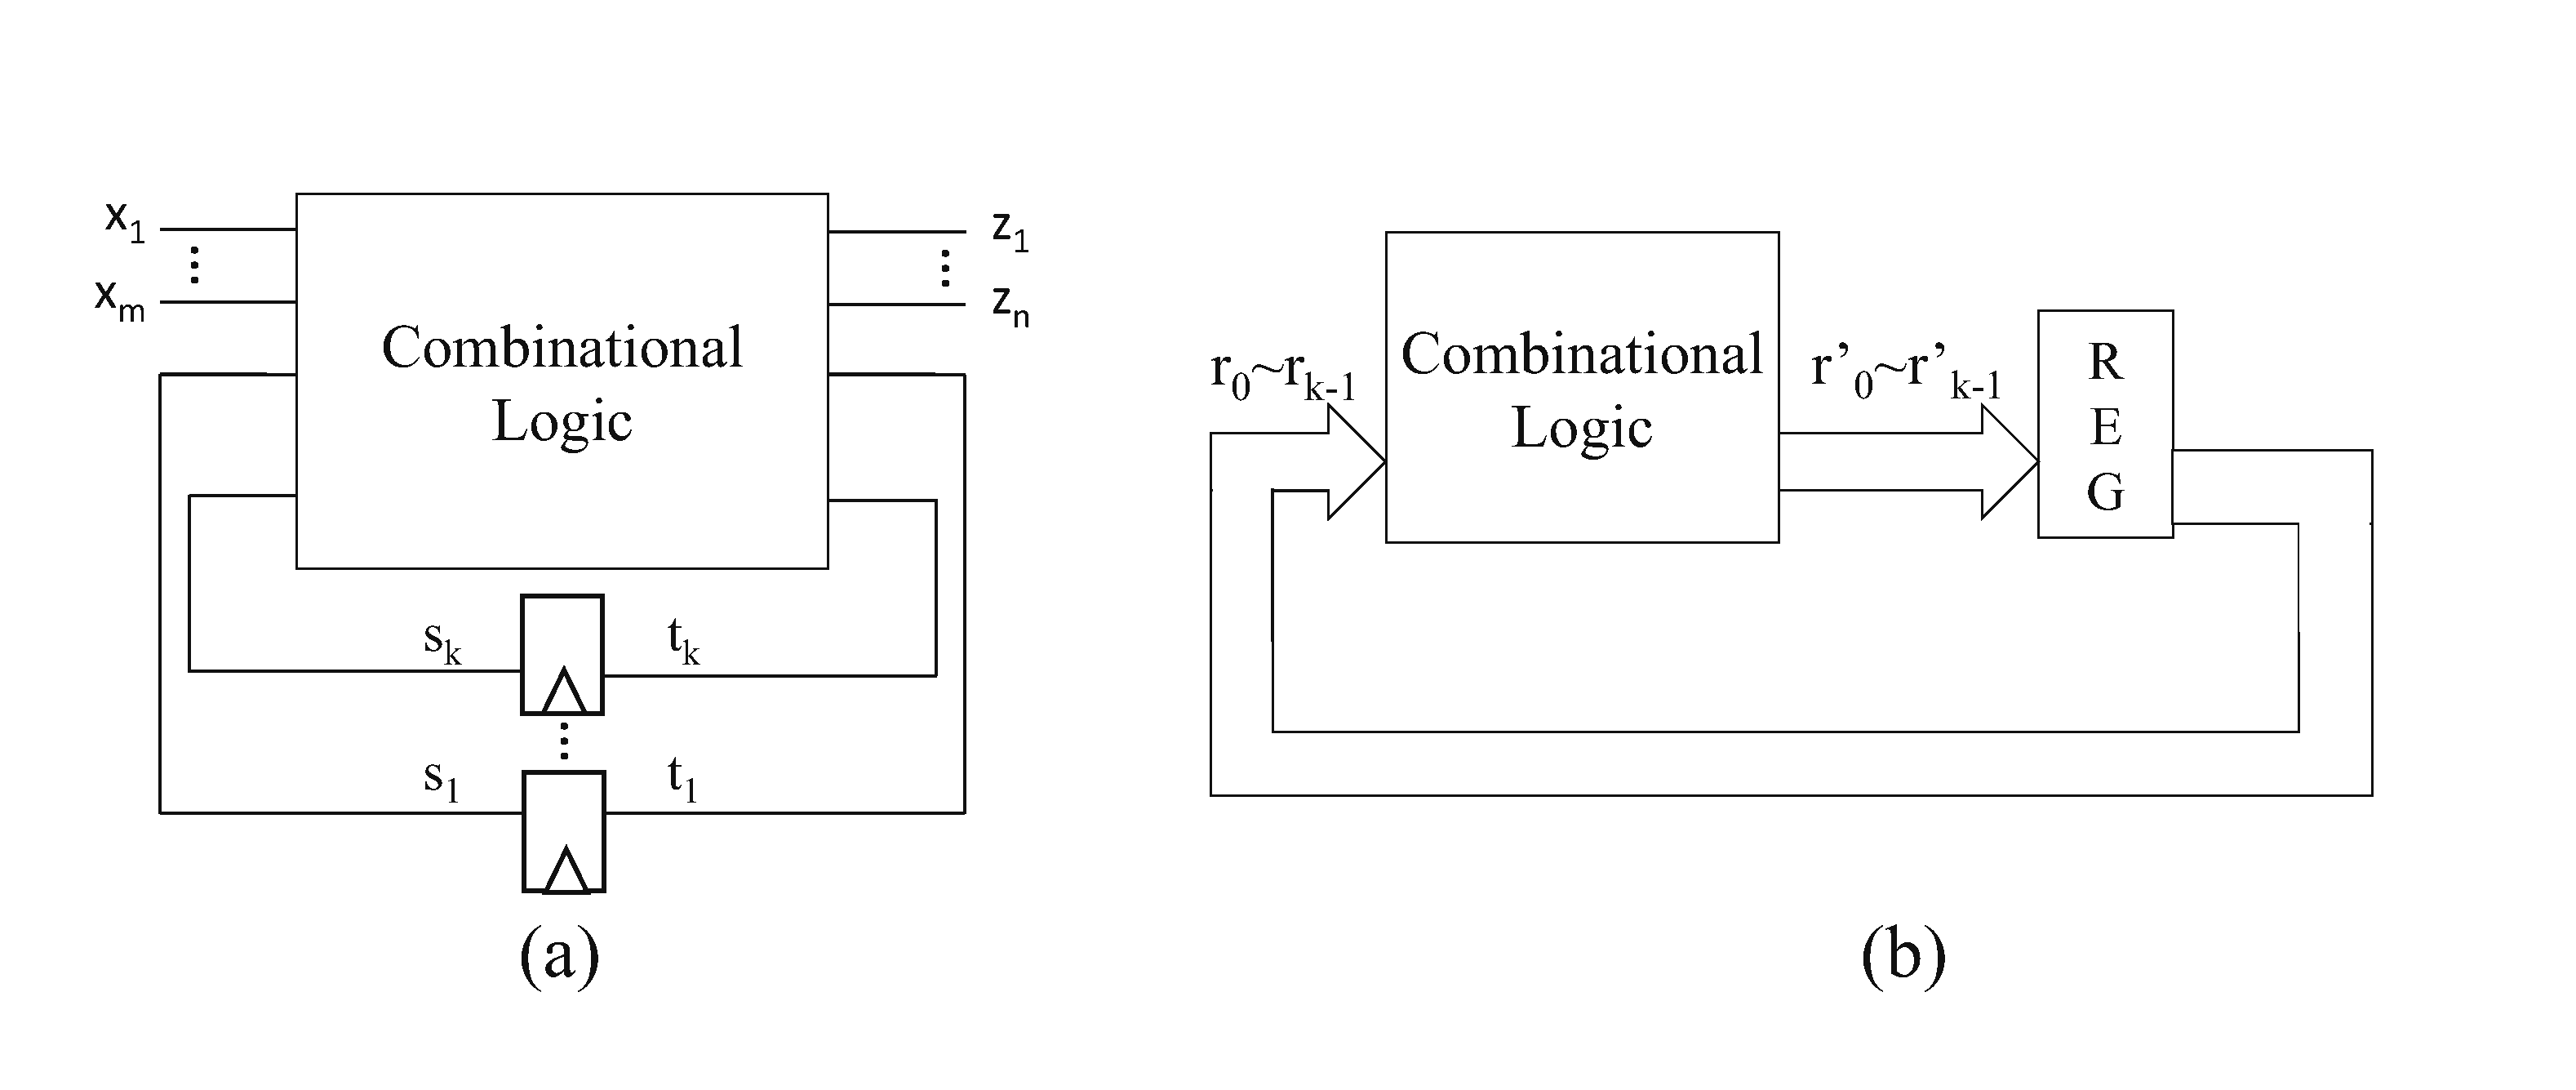
\includegraphics[width=\textwidth]{./seqmodel.eps}
 \vspace{-0.2in}
\caption{FSM models of sequential circuits}
\label{fig:seqmodel}}
\end{figure}
\bi
\item (a) A typical model for sequential circuits
\item (b) sequential datapath without primary inputs
\ei
\end{frame}

%%%%%%%%%%%%%%%%%%%%%%%%%%%%%%%%%%%%%%%%%%%%%%%%%%%%%%%
\begin{frame}{\large {State transition graph (STG) and breadth-first search (BFS) state space traversal}}
\begin{columns}[onlytextwidth]
\begin{column}{0.5\textwidth}
\begin{figure}
\centering
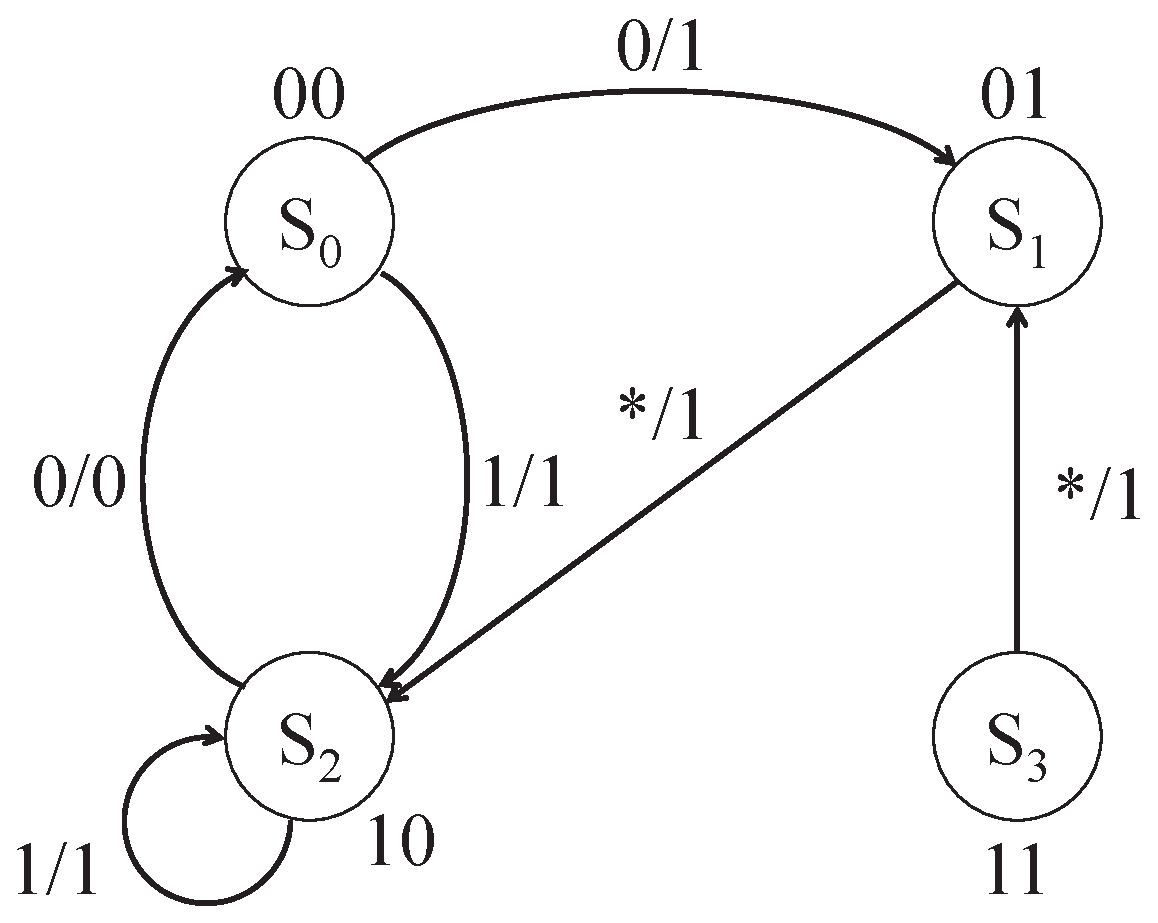
\includegraphics[scale=0.25]{stg_fig.eps}
\caption{State Transition Graph}
\end{figure}
\end{column}
\begin{column}{0.5\textwidth}
\bi
\item Initial state: $\{00\}$
\item Iteration 1: 
	\bi
	\item Start from $\{00\}$
	\item One-step transition: $\{01,10\}$
	\item Newly reached: $\{01,10\}$
	\ei
\item Iteration 2: 
	\bi
	\item Start from $\{01,10\}$
	\item One-step transition: $\{00,10\}$
	\item Newly reached: $\emptyset$
	\ei
\item All reachable states detected. Final reached states: $\{00,01,10\}$
\ei
\end{column}
\end{columns}

\end{frame}

%%%%%%%%%%%%%%%%%%%%%%%%%%%%%%%%%%%%%%%%%%%%%%%%

\begin{frame}{\large{BFS traversal with gate-level circuits}}
\begin{figure}[hbt]
\centerline{
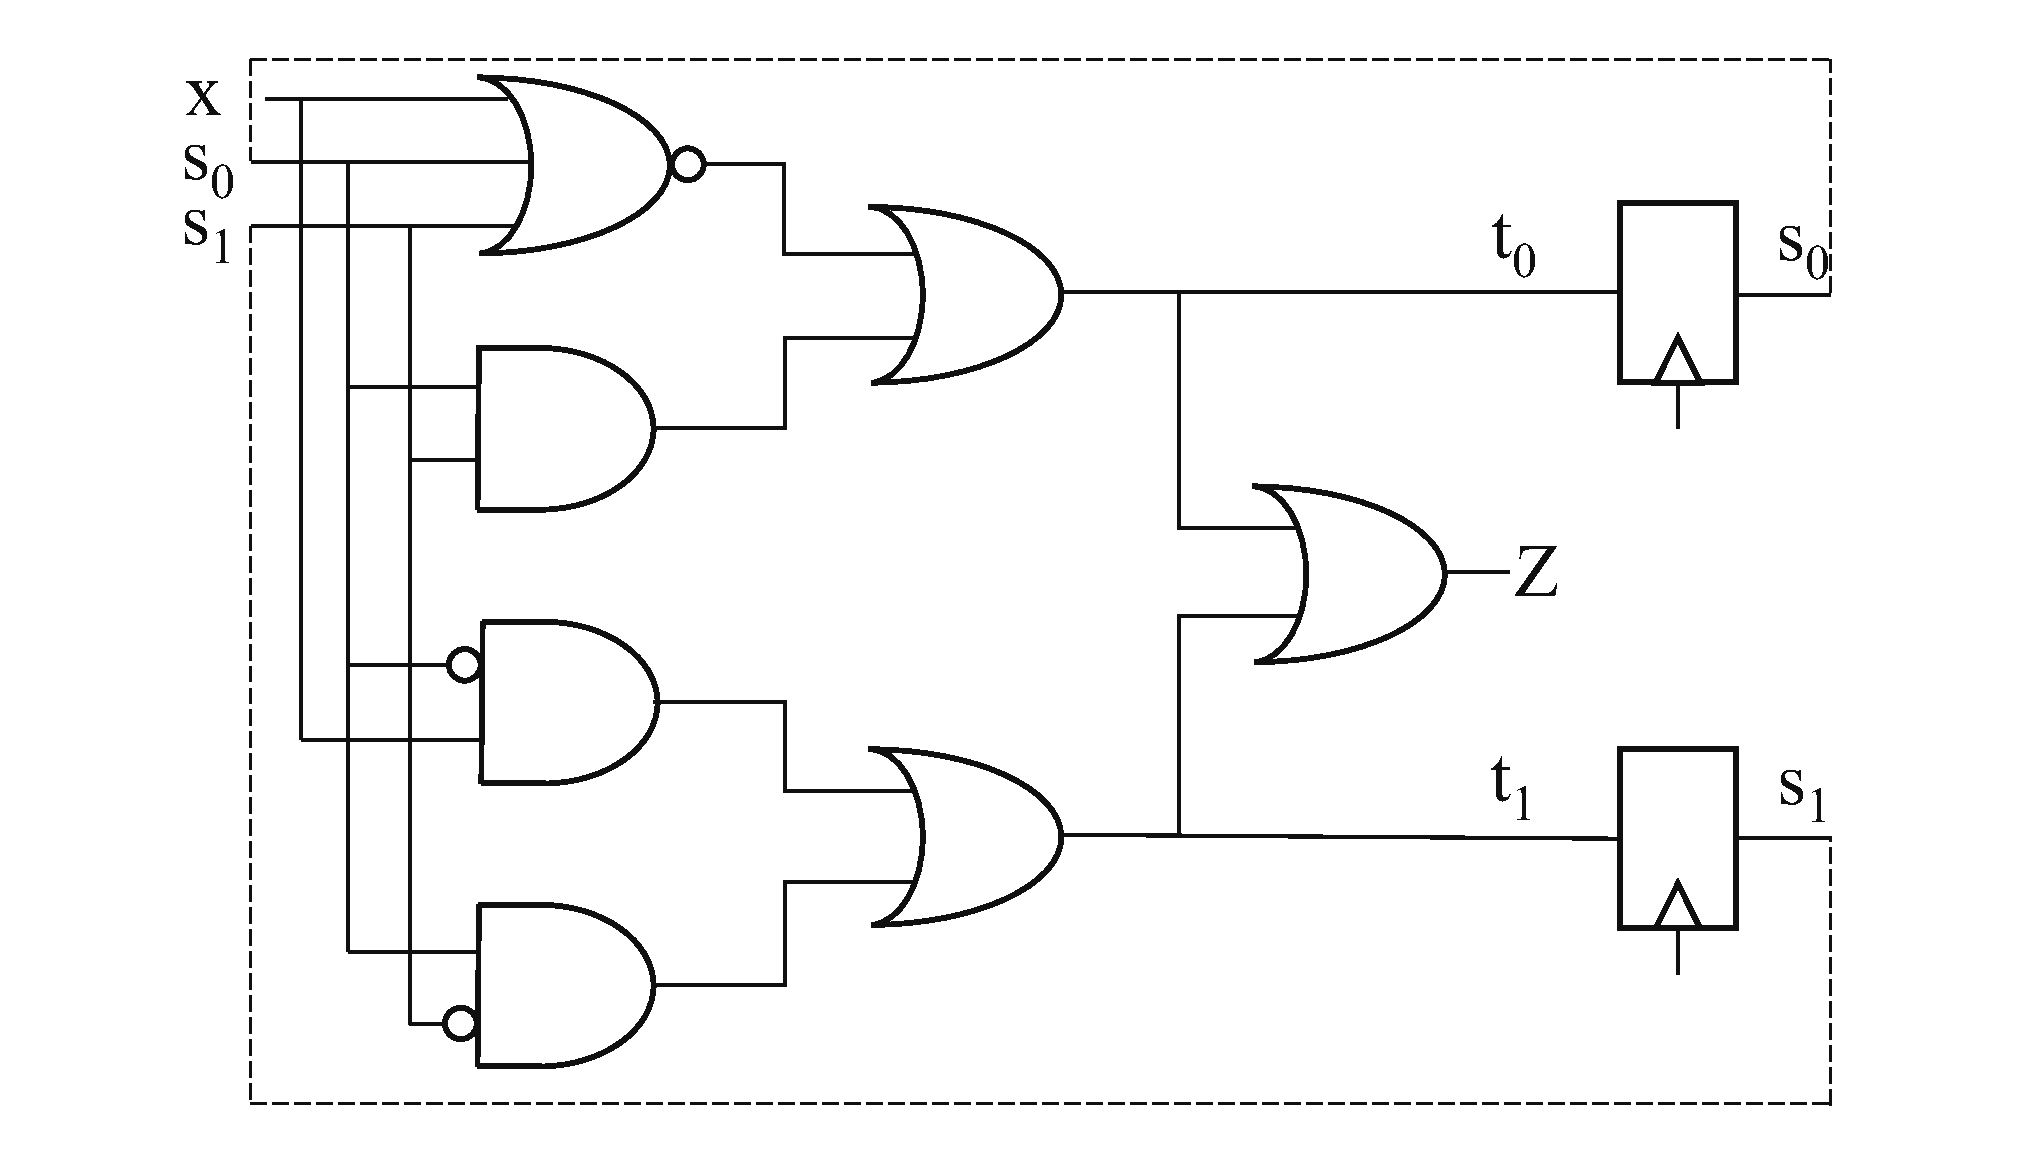
\includegraphics[scale=0.35]{fsm_fig.eps}
}
\caption{A Gate-level Circuit corresponding to last STG}
\end{figure}
An algorithmic approach is needed to implement BFS traversal
\end{frame}

%%%%%%%%%%%%%%%%%%%%%%%%%%%%%%%%%%%%%%%%%%%%%%%

\begin{frame}{\large{Breadth-First Traversal Algorithm based on Boolean formulas}}
\begin{algorithm}[H]
\SetAlgoNoLine
 \KwIn{Transition functions $\Delta$, initial state $S^0$}
  $from^0 = reached = S^0$\;
  \Repeat{$new^i == 0$}
  {
  	$i \gets i + 1$\;
	$to^i \gets$Img$(\Delta, from^{i-1})$\;
	$new^i \gets to^i \cap \overline{reached}$\;
  	$reached \gets reached \cup new^i$\;
	$from^i \gets new^i$\;
  }
\Return{$reached$}
\caption {Breadth-first Traversal Algorithm}
\end{algorithm}
\end{frame}

%%%%%%%%%%%%%%%%%%%%%%%%%%%%%%%%%%%%%%%%%%%%%%%

\begin{frame}{\large{Breadth-First Traversal Algorithm based on Boolean formulas(2)}}
\bi
\item Image function: $\text{Img}(\Delta, from) = \exists _s ~\exists _x ~[ T(s, x, t)
  \land from ] = \exists _s ~\exists _x ~\bigwedge_
  {i=1}^{n} (t_i
\overline{\oplus } \Delta_i)\land from$
\item Initial state: $from^0 = \overline{s_0}\land\overline{s_1}~(\{00\})$
\item Transition function: 
\begin{align*}
\Delta_1: & ~t_0 \overline{\oplus} ((\overline{x \lor s_0 \lor s_1}) ~\lor~ s_0\land s_1)\\
\Delta_2: & ~t_1 \overline{\oplus} (\overline{s_0}\land x ~\lor~ \overline{s_1}\land s_0)
\end{align*}
\item Iteration 1: 
	\bi
	\item One-step transition $to^1 = \exists _{s_0, s_1, x} (\Delta_1 \land \Delta_2
	\land from^0) = \overline{t_0}\land t_1~\lor~t_0\land \overline{t_1}~(\{01,10\})$
	\item Newly reached $new^1 = (\overline{t_0}\land t_1~\lor~t_0\land\overline{t_1})~\land ~
	\overline{(\overline{t_0}\land\overline{t_1})} = \overline{t_0}\land t_1~\lor~t_0\land\overline{t_1}$
	\ei
\item Iteration 2: same fashion
\item Return value: $reached = \{\overline{t_0}\lor \overline{t_1}\}~(\{00,01,10\})$
\ei
\end{frame}

%%%%%%%%%%%%%%%%%%%%%%%%%%%%%%%%%%%%%%%%%%%%%%%%%%
%%%%%%%%%%%%%%%%%%%%%%%%%%%%%%%%%%%%%%%%%%%%%%%%%%
\begin{frame}{\large{Outline}}
\bi
\item Introduction
\item Sequential circuit verification requires reachability analysis
\item From bit-level to word-level
	\bi
	\item \alert{All about math}
	\item Utilize the math tool: what does Tim get?
	\item My approach
	\ei
\item One step back: Sequential arithmetic circuit verification
\item New inspiration: UNSAT core extraction using algebraic geometry
\item The plan
\ei
\end{frame}
%%%%%%%%%%%%%%%%%%%%%%%%%%%%%%%%%%%%%%%%%%%%%%%%%%%
\begin{frame}{\large {Galois Field Overview}}
%\vspace{-0.2in}
%\ptsize{10}
\textbf {Galois field}(GF) $\mathbb{F}_q$ is a finite field with $q$
elements, $q = p^k$
\begin{itemize}
\item Commutative Ring with unity, associate, distributive laws
\item Closure property: $+,-,\times$, inverse ($\div$)
\end{itemize}

\begin{itemize}
\item $\mathbb{F}_p \equiv (\mathbb{Z} ~\pmod{ p })$, where $p = $ prime, is a field
\begin{itemize}
\item $\mathbb{Z}_7=\{0,1,2,3,4,5,6\}$
\end{itemize}


\end{itemize}

Our interest: $\mathbb{F}_{q} = \mathbb{F}_{2^k}$, i.e. $q = 2^k$
\begin{itemize}
\item  $\mathbb{F}_{2^k}$: $k$-dimensional extension of  $\mathbb{F}_{2}$
	\begin{itemize}
	\item $k$-bit bit-vector, AND/XOR arithmetic
	\end{itemize}
\end{itemize}

To construct $\mathbb{F}_{2^k}$
\begin{itemize}
\item $\mathbb{F}_{2^k} \equiv \mathbb{F}_{2}[x] \pmod {P(x)}$
\item $P(x) \in \mathbb{F}_{2}[x]$, irreducible polynomial of degree $k$
\end{itemize}

\end{frame}
%%%%%%%%%%%%%%%%%%%%%%%%%%%%%%%%%%%%%%%%%%%%%%%%%%
%%%%%%%%%%%%%%%%%%%%%%%%%%%%%%%%%%%%%%%%%%%%%%%%%%
%\begin{comment}

\begin{frame}{\large {Field Elements: {\it e.g.} $\mathbb{F}_8$}}
%\ptsize{10}

Consider: $\mathbb{F}_{2^3}= \mathbb{F}_{2}[x] \pmod {x^3 + x +
  1}$\\ $A \in \mathbb{F}_{2}[x]$ \\ 
$A \pmod {x^3 + x + 1} = a_2 x^2 + a_1 x + a_0$. Let $P(\alpha) = 0$:

\begin{itemize}
\item $\langle a_2, a_1, a_0 \rangle = \langle 0, 0, 0\rangle = 0$
\item $\langle a_2, a_1, a_0 \rangle = \langle 0, 0, 1\rangle = 1$
\item $\langle a_2, a_1, a_0 \rangle = \langle 0, 1, 0\rangle = \alpha$
\item $\langle a_2, a_1, a_0 \rangle = \langle 0, 1, 1\rangle = \alpha
  + 1$
\item $\langle a_2, a_1, a_0 \rangle = \langle 1, 0, 0\rangle = \alpha^2$
\item $\langle a_2, a_1, a_0 \rangle = \langle 1, 0, 1\rangle =
  \alpha^2 + 1$
\item $\langle a_2, a_1, a_0 \rangle = \langle 1, 1, 0\rangle =
  \alpha^2 + \alpha$
\item $\langle a_2, a_1, a_0 \rangle = \langle 1, 1, 1\rangle =
  \alpha^2 + \alpha + 1$
\end{itemize}
\end{frame}

%%%%%%%%%%%%%%%%%%%%%%%%%%%%%%%%%%%%%%%%%%%%%%%%%%%%%%%%%%%%%%%%
\begin{frame}{\large{Polynomial functions in Galois field}}
\bi
\item Polynomial functions over $\Fkk \Leftrightarrow$ Boolean functions on $k$-bit vectors
$$f:\B^k \to \B^k \Leftrightarrow \mathcal F:\Fkk \to \Fkk$$
\item Example: Lagrange's interpolation
\begin{figure}[H]
\centerline{
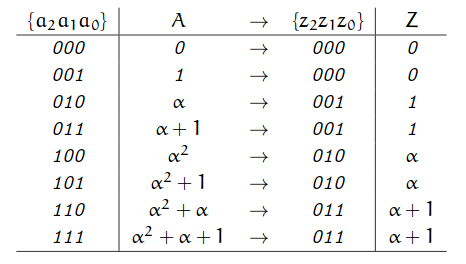
\includegraphics[scale=0.45]{lagrange.png}
}
%\caption{A Gate-level Circuit corresponding to last STG}
\end{figure}
\ei
\end{frame}
\begin{frame}{\large{Polynomial functions in Galois field(2)}}
\bi
\item 8 pairs of $(A,Z)$, use Lagrange's interpolation to abstract a polynomial function
$$Z = \F(A) = \sum_{n=1}^{8}\left[ \frac{\prod_{i\neq n}(A-A_i)}{\prod_{i\neq n}(A_n-A_i)}\cdot Z_n \right]$$
\item Result = $(\alpha^2+1)A^4+(\alpha^2+1)A^2~ implies$ \alert{polynomial representation of the function} 
\item $P(\alpha) = \alpha^3+\alpha+1 = 0$
\ei
\end{frame}
%%%%%%%%%%%%%%%%%%%%%%%%%%%%%%%%%%%%%%%%%%%%%%%%%%%%%%%%%%%%%%%%

\begin{frame}{\large{Algebraic Geometry Terminology}}
\vspace{-0.2in}
%\ptsize{10}
Let $\mathbb{F}_q = GF(2^k)$:
\begin{itemize}
\item $\mathbb{F}_q[x_1, \ldots, x_n]$: ring of all polynomials with
  coefficients in $\mathbb{F}_q$ 
\item Given a set of polynomials:
\begin{itemize}
\item $f, f_1, f_2, \dots , f_s \in \mathbb{F}_q[x_1, \dots, x_n]$
\item Find solutions to $f_1 = f_2 = \dots = f_s = 0$
\end{itemize}
\item \alert{Variety:} Set of ALL solutions to a given system of polynomial equations: $V(f_1, \dots, f_s)$
	\begin{itemize}
	\item In $\mathbb{R}\left[x,y\right]$, $V(x^2+y^2-1)=\{all\  points\  on\ circle: x^2+y^2-1=0\}$
	\item In $\mathbb{R}[x]$, $V(x^2+1)=\emptyset$
	\item In $\mathbb{C}[x]$, $V(x^2+1)=\{(\pm i)\}$
	\end{itemize}
\item Variety depends on the \alert{ideal} generated by the polynomials.
\item Reason about the Variety by analyzing the Ideals
\end{itemize}


\end{frame}
%%%%%%%%%%%%%%%%%%%%%%%%%%%%%%%%%%%%%%%%%%%%%%%%%%
%%%%%%%%%%%%%%%%%%%%%%%%%%%%%%%%%%%%%%%%%%%%%%%%%%

\begin{frame}{\large {Ideals and \Grobner basis}}
\vspace{-0.1in}


\begin{Definition}
{\bf Ideals of Polynomials:} Let $f_1, f_2, \ldots, f_s \in
\mathbb{F}_q[x_1, \dots, x_n]$. Let 
\begin{eqnarray}
J = \langle f_1, f_2 \ldots, f_s\rangle = \{f_1 h_1 + f_2 h_2 + \dots + f_s h_s\} \nonumber 
\end{eqnarray}

$J = \langle f_1, f_2 \ldots, f_s\rangle$ is an ideal generated by
$f_1, \ldots, f_s$ and the polynomials are called the generators. 
\end{Definition}

\vspace{-0.1in}
%\ptsize{10}

\begin{itemize}
\item Different generators can generate the same ideal
\item $\langle f_1,\cdots,f_s \rangle=\cdots=\langle g_1,\cdots,g_t
  \rangle$
\item Some generators are a ``better'' representation of the ideal
\item A (reduced){\bf Gr\"obner basis} is a ``canonical'' representation of an ideal
\end{itemize}

Given $F = \{f_1, f_2,\cdots, f_s\}$, Compute a Gr\"obner Basis (using Buchberger's algorithm) $G =
\{g_1,g_2,\cdots,g_t\}$, such that $I = \langle F \rangle = \langle G \rangle$

\begin{center}
$V(F)=V(G)$
\end{center}
\end{frame}

%%%%%%%%%%%%%%%%%%%%%%%%%%%%%%%%%%%%%%%%%%%%%%%%%%
%%%%%%%%%%%%%%%%%%%%%%%%%%%%%%%%%%%%%%%%%%%%%%%%%%
\begin{frame}{\large{Outline}}
\bi
\item Introduction
\item Sequential circuit verification requires reachability analysis
\item From bit-level to word-level
	\bi
	\item All about math
	\item \alert{Utilize the math tool: what does Tim get?}
	\item My approach
	\ei
\item One step back: Sequential arithmetic circuit verification
\item New inspiration: UNSAT core extraction using algebraic geometry
\item The plan
\ei
\end{frame}
%%%%%%%%%%%%%%%%%%%%%%%%%%%%%%%%%%%%%%%%%%%%%%%%%%%

\begin{frame}{\large {Elimination Theorem [Tim, {\it Abstraction using GB}, DAC'14]}}
\begin{itemize}
\item Let $J \subset \Fq[x_1,\dots,x_d]$ be an ideal
\end{itemize}
\begin{itemize}
\item Let $G$ be a \Grobner basis of $J$ with respect to a lex ordering where $x_1
> x_2 > \dots > x_d$.
\end{itemize}
\begin{itemize}
\item Then for every $0 \leq l \leq d$:
	\begin{itemize}	
	\item The set $G_l= G \cap \Fq[x_{l+1},\dots,x_d]$ is a Gr\"obner basis of the $l$th elimination ideal $J_l$.
	\end{itemize}
\end{itemize}

The $l$th elimination ideal does not contain variables
$x_1,\dots,x_l$, nor do the generators of it.

\end{frame}

%%%%%%%%%%%%%%%%%%%%%%%%%%%%%%%%%%%%%%%%%%%%%%%%%%

\begin{frame}{\large {Elimination Term Ordering Example}}
%\ptsize{10}
\begin{itemize}
\item Let ideal $I = \langle f_1, f_2, f_3 \rangle$ where
	\begin{itemize}
	\item $f_1 = x^2 + y + z - 1$
	\item $f_2 = x + y^2 + z - 1$
	\item $f_3 = x + y + z^2 - 1$
	\end{itemize}
\item The \Grobner basis of $I$ with lex order $(x > y > z)$ is
	\begin{itemize}
	\item $g_1 = x + y + z^2 - 1$
	\item $g_2 = y^2 - y - z^2 + z$
	\item $g_3 = 2yz^2 + z^4 - z^2$
	\item $g_4 = z^6 - 4z^4 + 4z^3 - z^2$
	\end{itemize}
\item Notice that $g_2$ and $g_3$ only contain variables $y$ and $z$
	\begin{itemize}
	\item Eliminates variable $x~\Leftrightarrow  ~\exists_x$ in Boolean formula!
	\end{itemize}
\item Similarly, $g_4$ only contains the variable $z$ and eliminates $x$ and $y$
\end{itemize}
\end{frame}

%%%%%%%%%%%%%%%%%%%%%%%%%%%%%%%%%%%%%%%%%%%%%%%%%%

\begin{frame}{\large {Abstraction Term Ordering[Tim, {\it Abstraction using GB}, DAC'14]}}

Derived from applying elimination theorem to our problem set
\begin{itemize}
\item Given a circuit $C$ implementing $Z = \F(A)$ over $\Fq$
\item Using the variable order $x_1 > x_2 > \dots > x_d > Z > A$
	\begin{itemize}
	\item $x_1, \dots ,x_d$ are the circuit variables
	\end{itemize}
\item Impose a lex term order $>$ on the polynomial ring $R = \Fq[x_1,
  \dots, x_d, Z, A]$.
\item This elimination term order $>$ is defined as
the {\bf Abstraction Term Order}.

\item Compute a Gr\"obner basis $G$ of ideal $(J
+ J_0)$ using $>$
	\begin{itemize}
	\item $G$ will contain a polynomial of the form $Z + \F(A)$ ($Z = \F(A)$)
	\item $Z = \F(A)$ is a \alert{unique, canonical, polynomial}
  representation of $C$ over $\Fq$ 
	\end{itemize}
\end{itemize}
\end{frame}

%%%%%%%%%%%%%%%%%%%%%%%%%%%%%%%%%%%%%%%%%%%%%%%%%%%%
\begin{frame}{\large{Abstraction Term Order Example}}

\centerline{
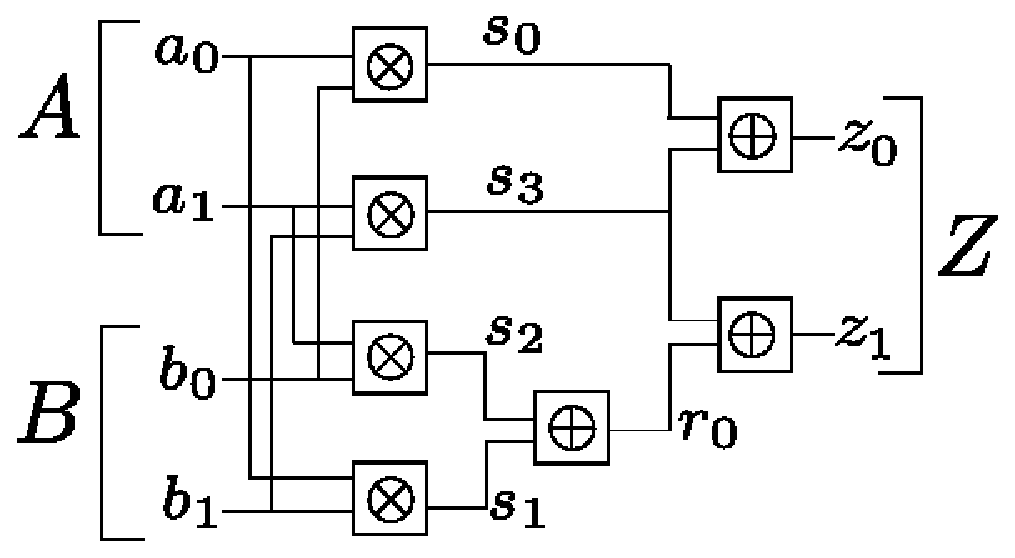
\includegraphics[scale=0.4]{2bitmult.eps}
}
%\vspace{-0.3in}
{\bf $(z_0 > z_1 > r_0 > s_0 > s_3 > s_1 > s_2 > a_0 > a_1 >  b_0 > b_1 > Z > A > B)$}
\begin{align*}
f_1: s_0+a_0 \cdot b_0; ~~f_2: s_1+a_0 \cdot b_1;  ~~f_3: s_2+a_1 \cdot b_0; ~~f_4: s_3+a_1 \cdot b_1  \nonumber \\
f_5: r_0+s_1 + s_2; ~~f_6: z_0+s_0 + s_3; ~~f_7: z_1+r_0+s_3; ~~f_8: a_0 + a_1 \alpha + A \nonumber \\ 
f_9: b_0 + b_1 \alpha + B; ~~f_{10}: z_0 + z_1 \alpha + Z \nonumber
\end{align*}
\vspace{-0.3in}
{\bf $J$ = $\langle f_1, \dots, f_{10} \rangle$}
\end{frame}

%%%%%%%%%%%%%%%%%%%%%%%%%%%%%%%

\begin{frame}{\large{Abstraction Term Order Example}}

\centerline{
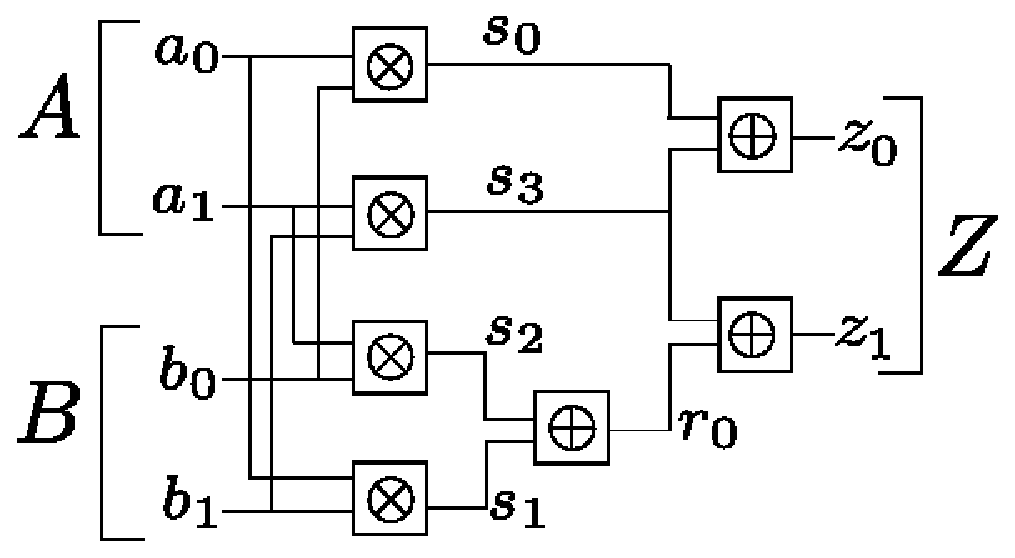
\includegraphics[scale=0.4]{2bitmult.eps}
}
%\vspace{-0.3in}
{\bf $(z_0 > z_1 > r_0 > s_0 > s_3 > s_1 > s_2 > a_0 > a_1 >  b_0 > b_1 > Z > A > B)$}
\begin{align*}
f_{11}: a_0^2+a_0; ~~f_{12}: a_1^2+a_1 \alpha; ~~f_{13}: b_0^2+b_0; ~~f_{14}: b_1^2+b_1; ~~f_{15}: s_0^2+s_0;  \nonumber \\
f_{16}: s_1^2+s_1; ~~f_{17}: s_2^2+s_2; f_{18}: s_3^2+s_3; ~~f_{19}: r_0^2+r_0; ~~f_{20}: z_0^2+z_0 \nonumber \\
f_{21}: z_1^2+z_1; ~~f_{22}: A^4+A; ~~f_{23}: B^4+B; ~~f_{24}:Z^4+Z \nonumber
\end{align*}
\vspace{-0.3in}
{\bf $J_0$ = $\langle f_{11}, \dots, f_{24} \rangle$}
\end{frame}

%%%%%%%%%%%%%%%%%%%%%%%%%%%%%%%

\begin{frame}{\large{Abstraction Term Order Example}}

\centerline{
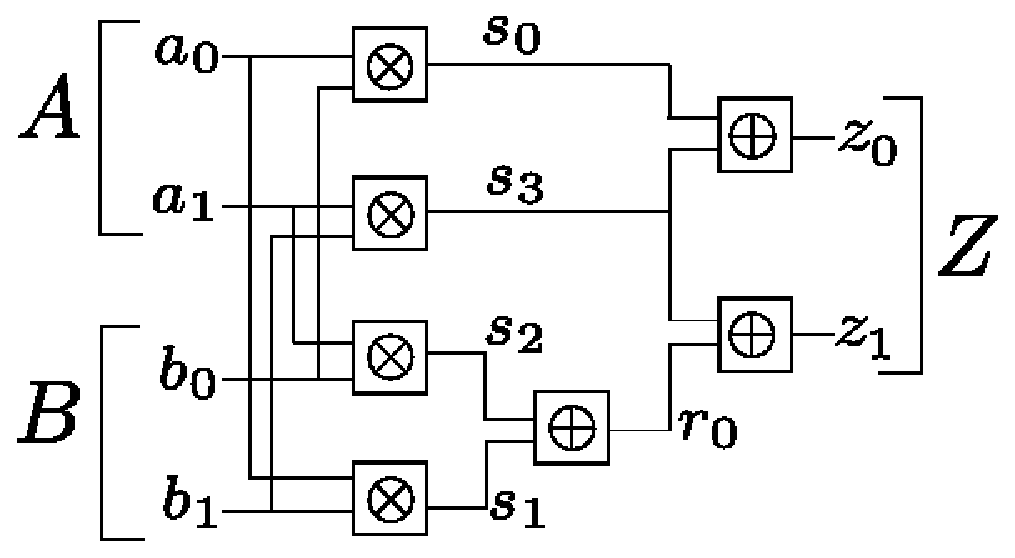
\includegraphics[scale=0.4]{2bitmult.eps}
}
%\vspace{-0.3in}
{\bf $(z_0 > z_1 > r_0 > s_0 > s_3 > s_1 > s_2 > a_0 > a_1 >  b_0 > b_1 > Z > A > B)$}

Compute the \Grobner basis, $G$, of \{$J + J_0$\} with respect to abstraction term ordering $>$.
$G$ = \{$g_1, \dots, g_{14}$\}
\begin{align*}
g_1: B^4+B; ~~g_2: b_0+b_1 \alpha + B; ~~g_3: a_0+a_1 \alpha + A; ~~g_4: A^4+A; \nonumber \\
g_5: s_0+s_1 \alpha + s_2 (\alpha + 1) + Z; ~~g_6: r_0+s_1+s_2; ~~g_7: z_1+r_0+s_3 \nonumber \\
g_7: z_0+z_1 \alpha +Z; ~~\alert{\bf g_9: Z+A*B} ; ~~g_{10}: b_1+B^2+B; ~~g_{11}: a_1+A^2+A \nonumber \\
g_{12}: s_3+a_1 b_1; ~~g_{13}: s_2+a_1 b_1 \alpha +a_1 B; ~~g_{14}: s_1+a_1 b_1 \alpha +b_1 A  \nonumber
\end{align*}

\end{frame}

%%%%%%%%%%%%%%%%%%%%%%%%%%%%%%
%%%%%%%%%%%%%%%%%%%%%%%%%%%%%%%%%%%%%%%%%%%%%%%%%%
\begin{frame}{\large{Outline}}
\bi
\item Introduction
\item Sequential circuit verification requires reachability analysis
\item From bit-level to word-level
	\bi
	\item All about math
	\item Utilize the math tool: what does Tim get?
	\item \alert{My approach}
	\ei
\item One step back: Sequential arithmetic circuit verification
\item New inspiration: UNSAT core extraction using algebraic geometry
\item The plan
\ei
\end{frame}
%%%%%%%%%%%%%%%%%%%%%%%%%%%%%%%%%%%%%%%%%%%%%%%%%%%


\begin{frame}{\large{Inspirations from Tim's work}}
 \vspace{-0.1in}
\begin{figure}[hbt]
\centering{
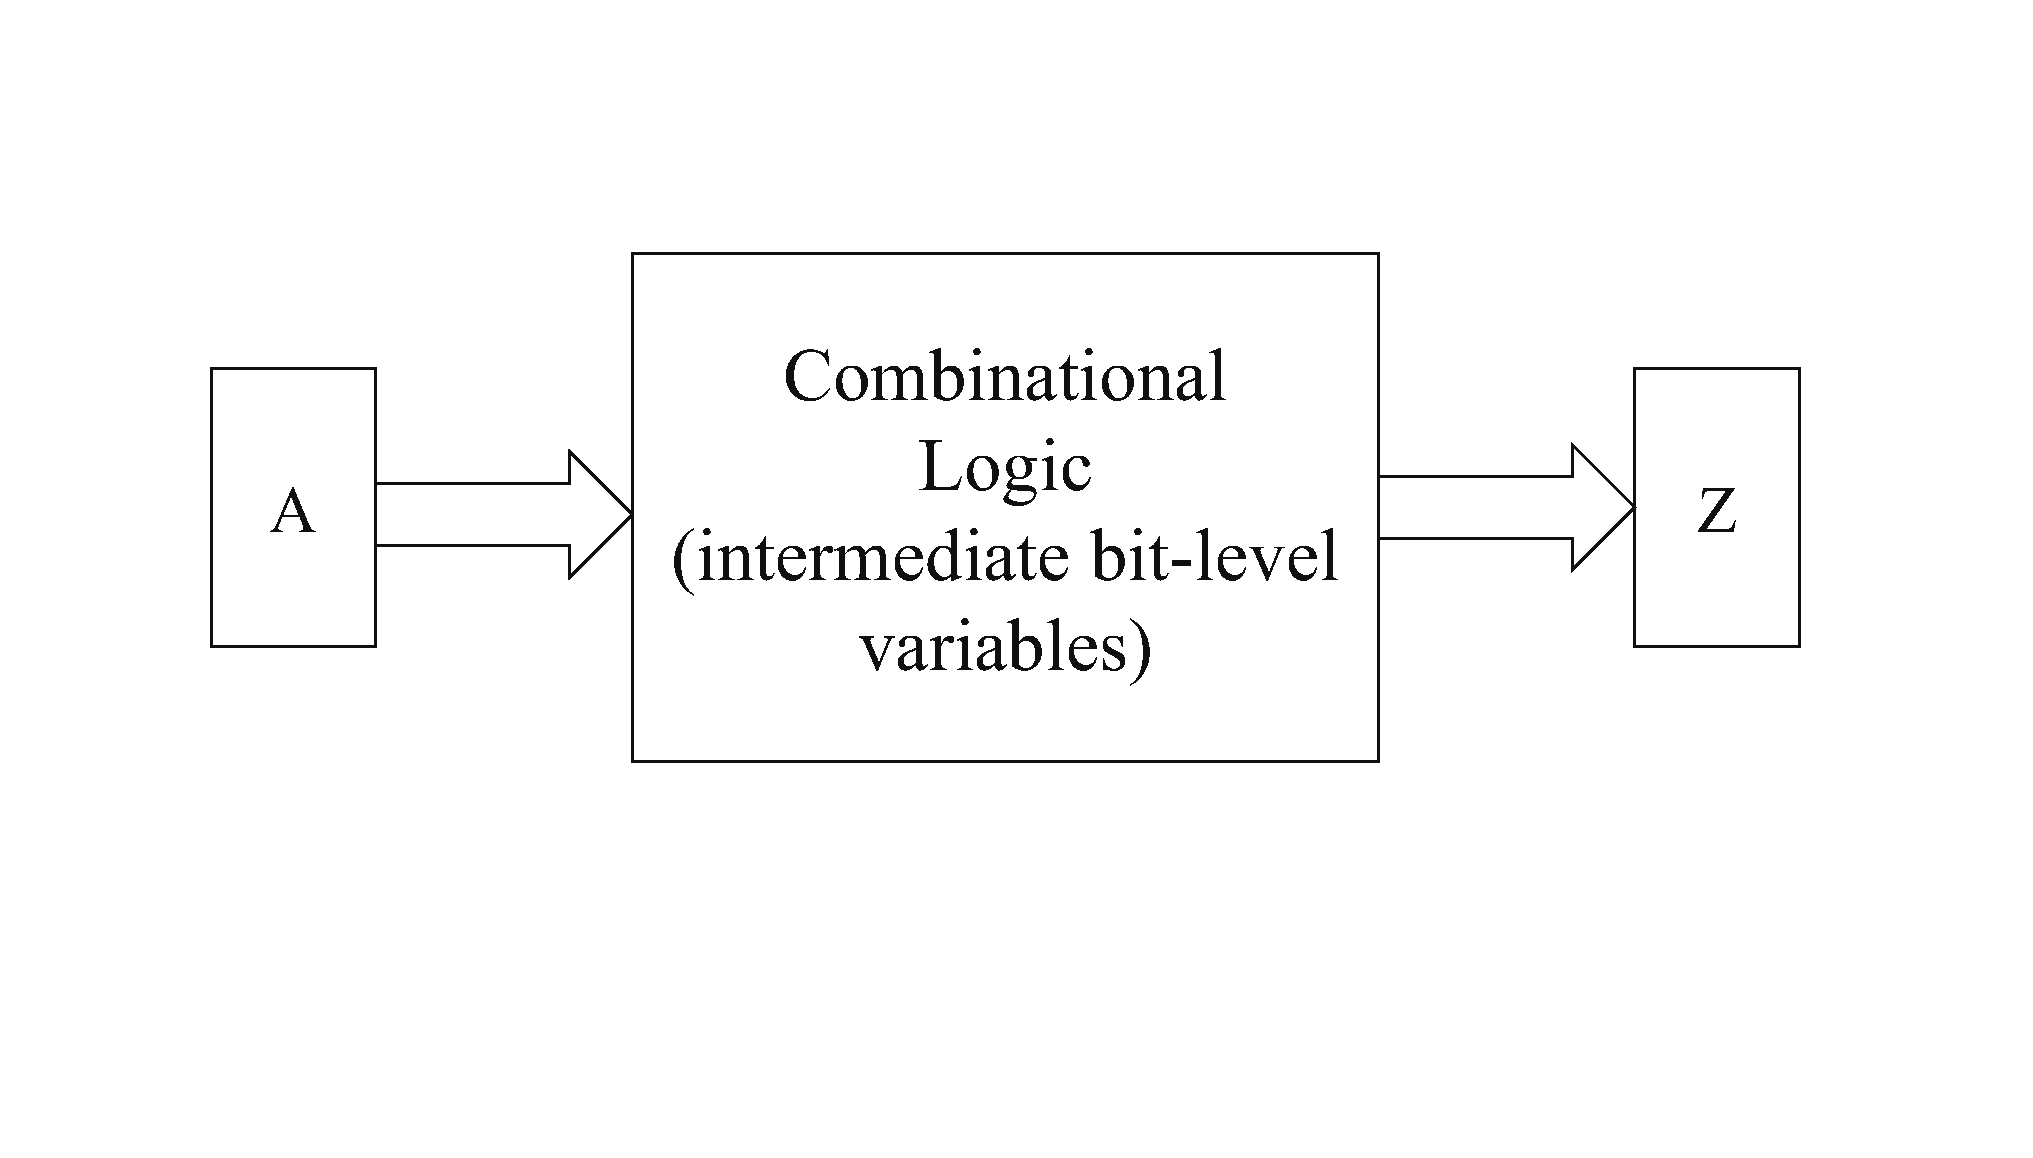
\includegraphics[width=\textwidth]{./comb2.eps}
%\caption{FSM models of sequential circuits}
\label{fig:comb}}
\end{figure}
 \vspace{-1in}
\bi
\item From Tim's work I learned:
	\bi
	\item Compute GB with term order {\it intermediate $>$ Z $>$ A}
	\item Obtain $Z = \mathcal F(A)$
	\ei
\item Inspiration: what if we impose term order {\it intermediate $>$ A $>$ Z} ?
\item Proposed approach: add the evaluation of $A$ into elimination ideal, then eliminate all but $Z$, we will get the 
\alert{evaluation of $Z$}!
	\bi
	\item Present state $\gets A$, next state $\gets Z$
	\item It is a way to do \alert{one-step reachability}!
	\ei
\ei
\end{frame}

%%%%%%%%%%%%%%%%%%%%%%%%%%%%%%%%%%%%%%%%%%%%%%%%%%%%%%
\begin{frame}{\large{Recall: Breadth-First Traversal Algorithm}}
\begin{algorithm}[H]
\SetAlgoNoLine
 \KwIn{Transition functions $\Delta$, initial state $S^0$}
  $from^0 = reached = S^0$\;
  \Repeat{$new^i == 0$}
  {
  	$i \gets i + 1$\;
	$to^i \gets$Img$(\Delta, from^{i-1})$\;
	$new^i \gets to^i \cap \overline{reached}$\;
  	$reached \gets reached \cup new^i$\;
	$from^i \gets new^i$\;
  }
\Return{$reached$}
\caption {Breadth-first Traversal Algorithm}
\end{algorithm}
\vspace{0.2in}
\textbf{We want to implement this algorithm using algebraic geometry approach}
\end{frame}

%%%%%%%%%%%%%%%%%%%%%%%%%%%%%%%%%%%%%%%%%%%%%%%%%%%%%%

\begin{frame}{\large{Implement Image Function in Algebraic Geometry}}
\begin{itemize}
\item State variables (word-level) $S, T$ and sets of states such as
$from^i, to^i$ can always be represented as varieties of ideals.
\item Boolean operators can always be converted to operations in $\mathbb F_2$
\begin{table}
\centering
\begin{tabular}{|c|c|} \hline
Boolean operator & operation in $\mathbb{F}_{2}$\\ \hline
$\overline{a}$ & $1 + a$\\ \hline
$a\ and\ b$ & $ab$\\ \hline
$a\ or\ b$ & $a + b + ab$\\ \hline
$a \oplus b$ & $a + b$\\
\hline\end{tabular}
\caption{Some Boolean operators and corresponding operations in $\mathbb{F}_{2}$}
\label{table:booltogalois_op}
\end{table}
\item An \emph{elimination ideal} can be built from circuit gates, PS/NS
word definition and vanishing polynomials
\end{itemize}
\end{frame}

%%%%%%%%%%%%%%%%%%%%%%%%%%%%%%%%%%%%%%%%%%%%%%%%%%
\begin{frame}{\large {Example Formulation}}
\vspace{-0.1in}
\begin{figure}[hbt]
\centerline{
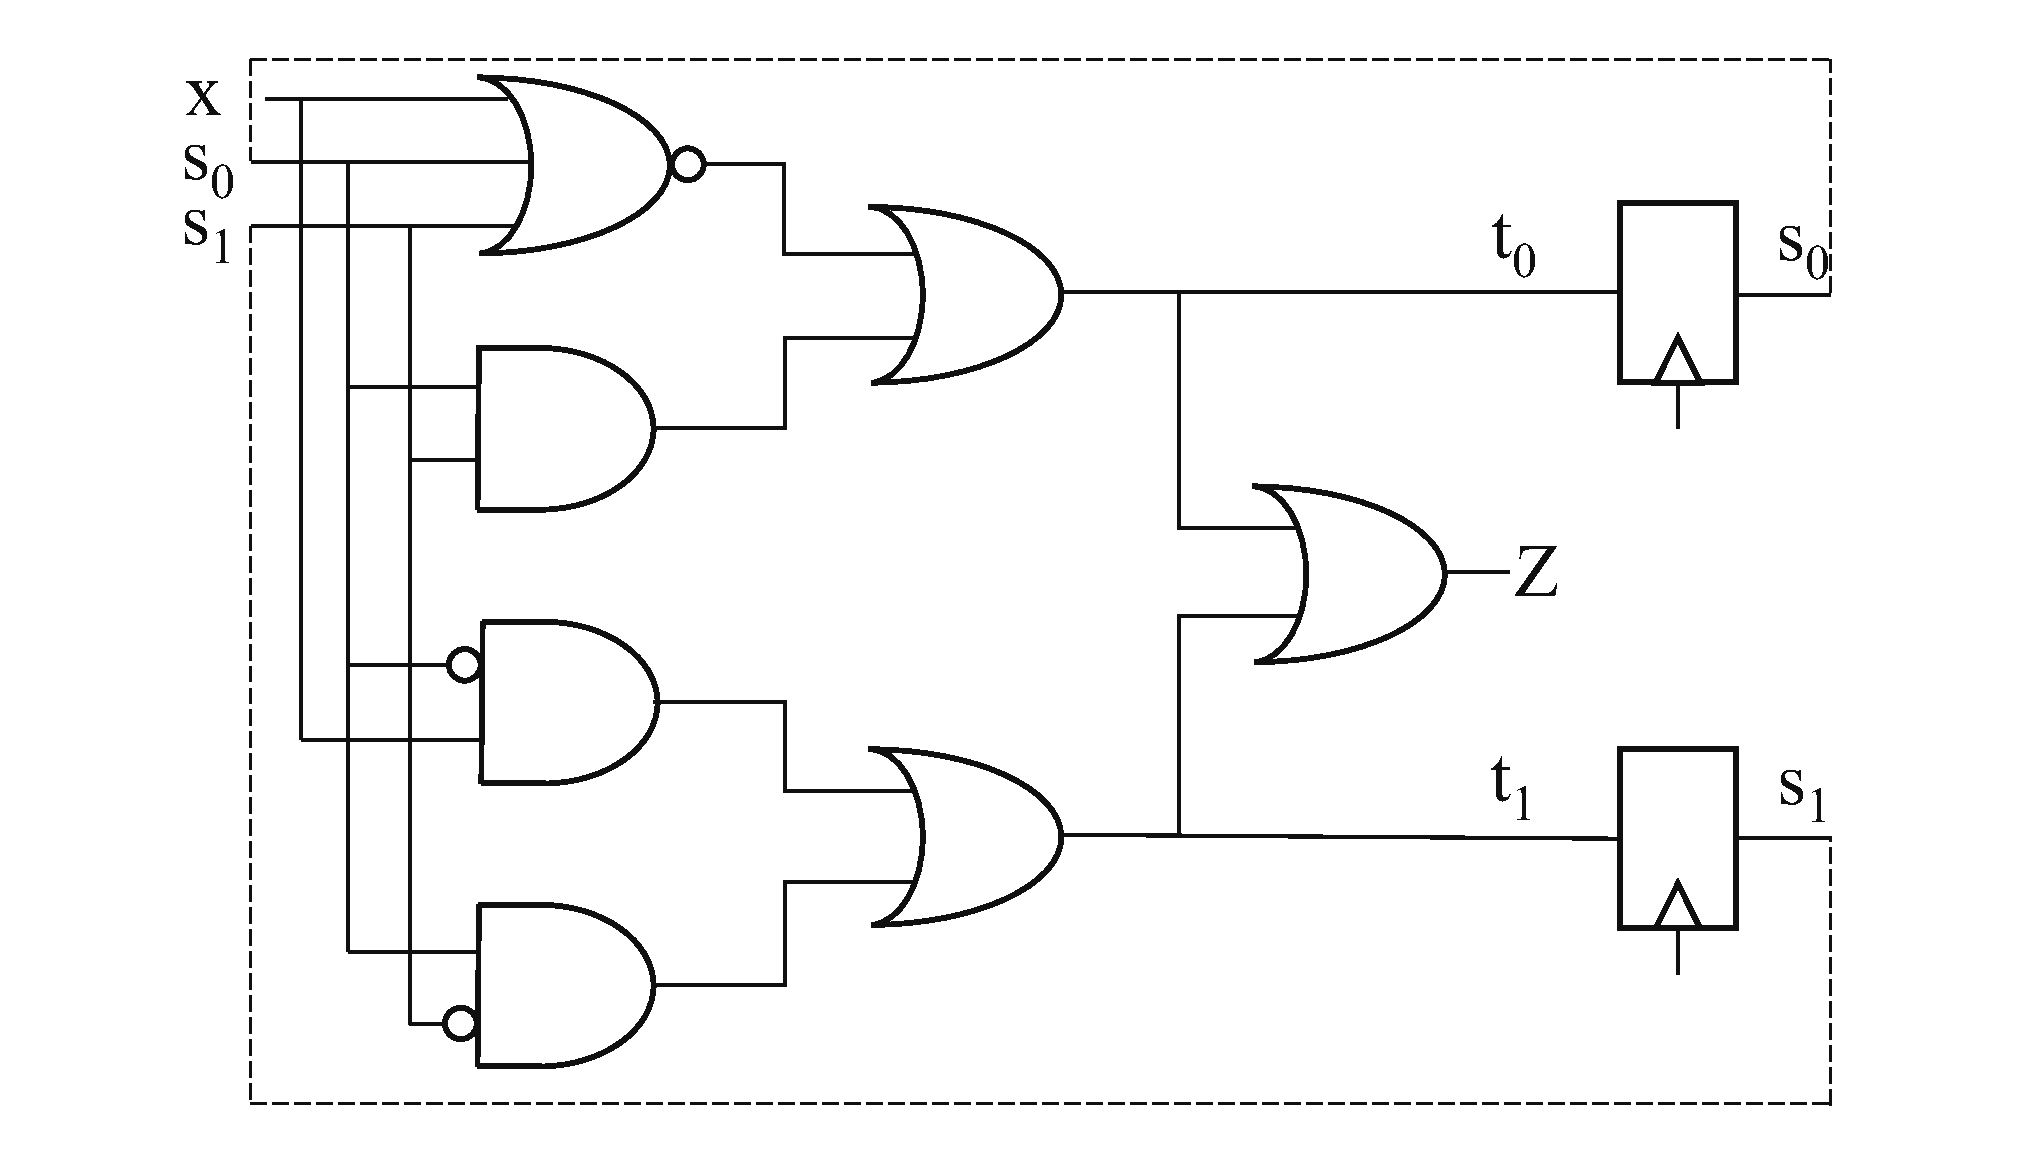
\includegraphics[scale=0.25]{fsm_fig.eps}
}
%\caption{A multiplier over GF($2^2$)}
%\label{fig:fsm}
\end{figure}
\vspace{-0.4in}
Model circuit as polynomials in $\mathbb{F}_2 \subset \mathbb{F}_{2^k}$:
\begin{align*}
&t_0 = (\overline{x}\ and\ \overline{s_0}\ and\ \overline{s_1})\ or\ (s_0\ and\ s_1)\\
&\implies f_1: t_0- (xs_0s_1+xs_0+xs_1+x+s_0+s_1+1)\\
&t_1 = (\overline{s_0}\ and\ x)\ or\ (s_0\ and\ \overline{s_1})~~~~\\
&\implies f_2: t_1 - (xs_0+x+s_0s_1+s_0)\\
&f_3: S + s_0 + s_1\alpha, ~~f_4:T + t_0 + t_1\alpha
\end{align*}
\end{frame}
%%%%%%%%%%%%%%%%%%%%%%%%%%%%%%%%%%%%%%%%%%%%%%%%%%%%%%%%%%%
\begin{frame}{\large{Example Formulation(2)}}
\bi
\item Elimination ideal to model Image function for example circuit:
\begin{itemize}
\item Transition functions (bit-level): $f_1,f_2$\\

\item Word variable definitions: $f_3,f_4$\\

\item Vanishing polynomials: $f_6: x^2 - x; f_7: t_0^2 - t_0; f_8: t_1^2 - t_1; f_9: S^4 - S; f_{10}: s_0^2 - s_0;
f_{11}: s_1^2 - s_1; f_{12}: T^4 - T$
\end{itemize}
\item Add the present state (e.g. initial states in first iteration $f_5: S$), compute Gr\"obner basis
for ideal $J = \langle f_1,\dots, f_{12}\rangle$ under elimination term order $$intermediate\ bit\text{-}level\ signals >\ bit\text{-}level\ PIs/POs >\ S >\ T$$
\item  Result will include a univariate polynomial about \emph{next states} $T$, e.g. $T^2+(\alpha+1)T+\alpha$ 
\ei
\end{frame}

%%%%%%%%%%%%%%%%%%%%%%%%%%%%%%%%%%%%%%%%%%%%%%%%%%%%%%%%%%%
\begin{frame}{\large{Recall: Breadth-First Traversal Algorithm}}
\begin{algorithm}[H]
\SetAlgoNoLine
 \KwIn{Transition functions $\Delta$, initial state $S^0$}
  $from^0 = reached = S^0$\;
  \Repeat{$new^i == 0$}
  {
  	$i \gets i + 1$\;
	$to^i \gets$Img$(\Delta, from^{i-1})$\;
	$new^i \gets to^i \cap \overline{reached}$\;
  	$reached \gets reached \cup new^i$\;
	$from^i \gets new^i$\;
  }
\Return{$reached$}
\caption {Breadth-first Traversal Algorithm}
\end{algorithm}
\vspace{0.2in}
\textbf{We want to implement this algorithm using algebraic geometry approach}
\end{frame}
%%%%%%%%%%%%%%%%%%%%%%%%%%%%%%%%%%%%%%%%%%%%%%%%%%%%%%%%%%%

\begin{frame}{\large{Intersection and union in algebraic geometry}}
\begin{Definition}
\label{def:sum}
({\bf Sum/Product of Ideals}) If $I = \langle f_1, \dots, f_r\rangle$ and $J = \langle g_1, \dots, g_s\rangle$ are 
ideals in $\mathbb F[x_1, \dots, x_n]$, then the {\bf sum} of $I$ and $J$ is defined as
$$I + J = \langle f_1, \dots, f_r, g_1, \dots, g_s\rangle$$ And the {\bf product} of $I$ and $J$ is defined
as
\begin{equation}
  I \cdot J = \langle f_ig_j\ |\ 1 \leq i \leq r, 1 \leq j \leq s\rangle \nonumber
  \end{equation}
\end{Definition}
\begin{Theorem}
\label{thm:unionintersect}
If $I$ and $J$ are ideals in $\mathbb F[x_1, \dots, x_n]$, then ${\bf
  V}(I + J) = {\bf V}(I) \bigcap {\bf V}(J)$ and ${\bf V}(I \cdot J) =
{\bf V}(I) \bigcup {\bf V}(J)$. 
\end{Theorem}
\end{frame}

%%%%%%%%%%%%%%%%%%%%%%%%%%%%%%%%%%%%%%%%%%%%%%%%%%%%%%%%%%
\begin{frame}{\large{Complement set in algebraic geometry}}
\begin{Definition}
({\bf Quotient of Ideals}) If $I$ and $J$ are ideals in $\mathbb
  F[x_1, \dots, x_n]$, then $I:J$ is the set
  \begin{equation}
  \{f \in \mathbb F[x_1, \dots, x_n]\ |\ f\cdot g \in I, \forall g \in J\}\nonumber
  \end{equation}
and is called the {\bf ideal quotient} of $I$ by $J$.
\end{Definition}
\begin{Theorem}
\label{thm:quotient}
Let $I, J$ be ideals with vanishing polynomials over $\Fkk[x_1,\dots,x_n]$, then 
$${\bf V}(I:J) = {\bf V}(I) - {\bf V}(J)$$
\end{Theorem}
\end{frame}

%%%%%%%%%%%%%%%%%%%%%%%%%%%%%%%%%%%%%%%%%%%%%%%%%%%%%%%%%%%%
\begin{frame}[label = pptalg]{\large{Our proposed algorithm of BFS traversal based on algebraic geometry}}
\begin{algorithm}[H]
\SetAlgoNoLine
 \KwIn{Input-output circuit characteristic polynomial ideal $J_{ckt}$, initial state polynomial $\F(S)$}
  $from^0 = reached = \F(S)$\;
  \Repeat{$new^i == 1$}
  {
  	$i \gets i + 1$\;
	$to^i \gets$GB w/ elimination term order$\langle J_{ckt},J_0, from^{i-1}\rangle$\;
	$new^i \gets $generator of $\langle to^i\rangle + (\langle T^4-T\rangle:\langle reached\rangle)$\;
  	$reached \gets $generator of $\langle reached\rangle \cdot \langle new^i\rangle$\;
	$from^i \gets new^i(S\setminus T)$\;
  }
\Return{$reached$}
\caption{Algebraic Geometry based Traversal Algorithm}
\end{algorithm}

\hyperlink{pptpage2}{\beamergotobutton{Go to example page 2}}

\hyperlink{pptpage3}{\beamergotobutton{Go to example page 3}}
\end{frame}

%%%%%%%%%%%%%%%%%%%%%%%%%%%%%%%%%%%%%%%%%%%%%%%%%%%%%%%%%%%%
\begin{frame}{\large{Full Blown traversal of example circuit using algebraic geometry}}
\bi
\item Initial state $from^0 = S(\{00\})$
\item {\bf Iteration 1:}Compose an elimination ideal $J$ 
\vspace{-0.2in}\\
\begin{align*}
&f_1: t_0- (xs_0s_1+xs_0+xs_1+x+s_0+s_1+1)\\
&f_2: t_1 - (xs_0+x+s_0s_1+s_0)\\
&f_3: S - s_0 - s_1\\
&f_4: T - t_0 - t_1
\end{align*}
$J_{ckt} = \langle f_1,f_2,f_3,f_4\rangle$
\begin{align*}
&f_5: x^2-x\\
&f_6: s_0^2-s_0, f_7: s_1^2-s_1\\
&f_8: t_0^2-t_0, f_9: t_1^2-t_1\\
&f_{10}: S^4-S, f_{11}:T^4-T
\end{align*}
$\ \ \ \ \ \ \ \ \ \ \  \ J_0 = \langle f_5,f_6,\dots,f_{11}\rangle$
\ei
\end{frame}
%%%%%%%%%%%%%%%%%%%%%%%%%%%%%%%%%%%%%%%%%%%%%%%%%%%%%%%%%%%
\begin{frame}[label = pptpage2]
\bi
\item Elimination term order: 
$$\{x,s_0,s_1,t_0,t_1\}~(all~bits)~>~S~(PS~word)~ >~ T~(NS~word)$$
\item Compute the reduced GB for $J = J_{ckt}+J_0+\langle from^0\rangle$
\item Next state 
$$to^1 = \langle T^2+(\alpha+1)T+\alpha\rangle~(\{01,10\})$$
\item Complement of formerly reached state:
$$\langle T^4-T\rangle:\langle T\rangle = \langle T^3+1\rangle ~(\{01,10,11\})$$
\item Newly reached state:
$$\langle T^3+1, T^2+(\alpha+1)T+\alpha \rangle = \langle T^2+(\alpha+1)T+\alpha \rangle$$ 
\item Update current reached states 
$$reach = \langle T\cdot T^2+(\alpha+1)T+\alpha \rangle = \langle T^3+(\alpha+1)T^2+\alpha T\rangle~(\{00,01,10\})$$
\item Update the present states for next iteration
$$from^1 = \langle S^2+(\alpha+1)S+\alpha\rangle$$
\ei
\hyperlink{pptalg}{\beamergotobutton{The algorithm}}
\end{frame}
%%%%%%%%%%%%%%%%%%%%%%%%%%%%%%%%%%%%%%%%%%%%%%%%%%%%%%%%%%%
\begin{frame}[label = pptpage3]{\large{Full Blown traversal of example circuit using algebraic geometry(3)}}
\bi
\item Iteration 2:
	\bi
	\item Next state: $to^2 = \langle T^2+\alpha T\rangle~(\{00,10\})$
	\item The complement of $reached$:
	$$\langle T^4-T\rangle:\langle T^3+(\alpha+1)T^2+\alpha T\rangle
= \langle T + 1+\alpha\rangle ~(\{11\})$$ 
	\item Newly reached state: 
$$\langle T^2+\alpha T, T+1+\alpha \rangle = \langle \alert{1}\rangle$$ 
	\ei
\item Algorithm terminates
\item Return value (final reachable states):
$$reached = \langle T^3+(\alpha+1)T^2+\alpha T\rangle$$
\ei
\hyperlink{pptalg}{\beamergotobutton{The algorithm}}
\end{frame}

%%%%%%%%%%%%%%%%%%%%%%%%%%%%%%%%%%%%%%%%%%%%%%%%%%
\begin{frame}{\large{Outline}}
\bi
\item Introduction
\item Sequential circuit verification requires reachability analysis
\item From bit-level to word-level
\item \alert{One step back: Sequential arithmetic circuit verification}
\item New inspiration: UNSAT core extraction using algebraic geometry
\item The plan
\ei
\end{frame}
%%%%%%%%%%%%%%%%%%%%%%%%%%%%%%%%%%%%%%%%%%%%%%%%%%%
%%%%%%%%%%%%%%%%%%%%%%%%%%%%%%%%%%%%%%%%%%%%%%%%%%%%%%%%%%%%
\begin{frame}{\large{Application on implicit unrolling}}
\vspace{-0.1in}
\begin{figure}[hbt]
\centering{
%\begin{minipage}{12cm}
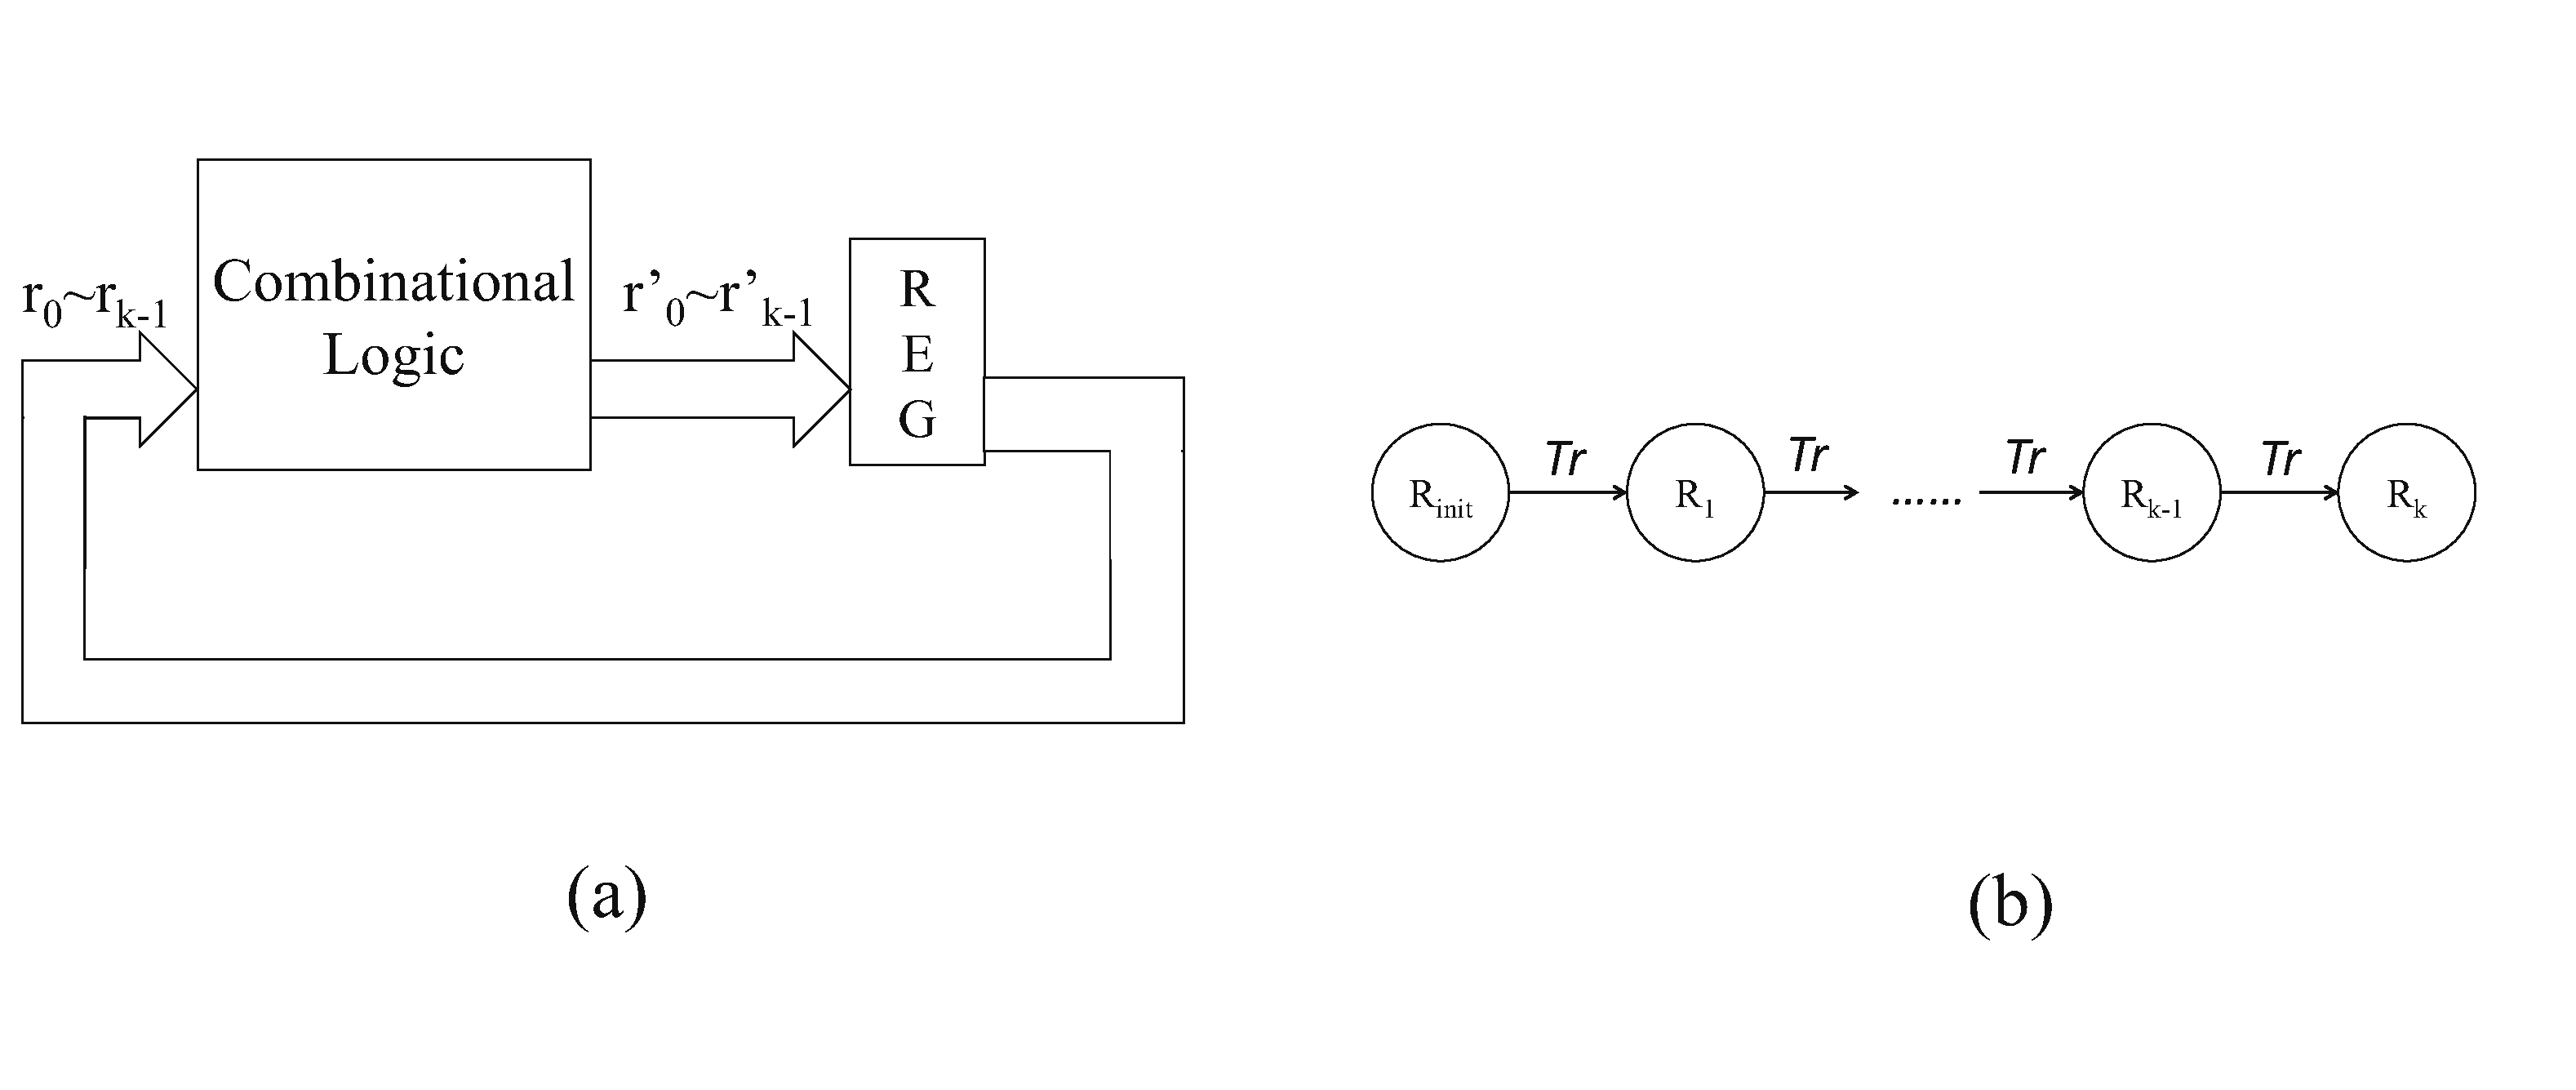
\includegraphics[width=4.5in]{./Moore.eps}
% \vspace{-0.2in}
%\caption{A simple Moore FSM and its state transition graph}
%\end{minipage}
\label{fig:Moore}}
\end{figure}
\vspace{-0.2in}
\bi
\item State enumeration cannot address sequential arithmetic circuits verification
	\bi
	\item Need to consider various initial states
	\item Exact reached states after $k$ clock cycles directly implies desired arithmetic function
	\ei
\item State transitions on simplified model
$$R_{k} = Tr(R_{k-1}) = Tr(Tr(\cdots Tr(R_{init})\cdots)) = Tr^k(R_{init})$$
\ei
\end{frame}
%%%%%%%%%%%%%%%%%%%%%%%%%%%%%%%%%%%%%%%%%%%%%%%%%%%%%%%%%%
\begin{frame}{\large{Verification of a sequential Galois field multiplier (Normal basis)}}
SPEC: $R = A_{init}\cdot B_{init} \pmod {P(\alpha)}$ after $k$ clock cycles
\hspace{-0.3in}\begin{figure}[hbt]
\centering{
%\begin{minipage}{12cm}
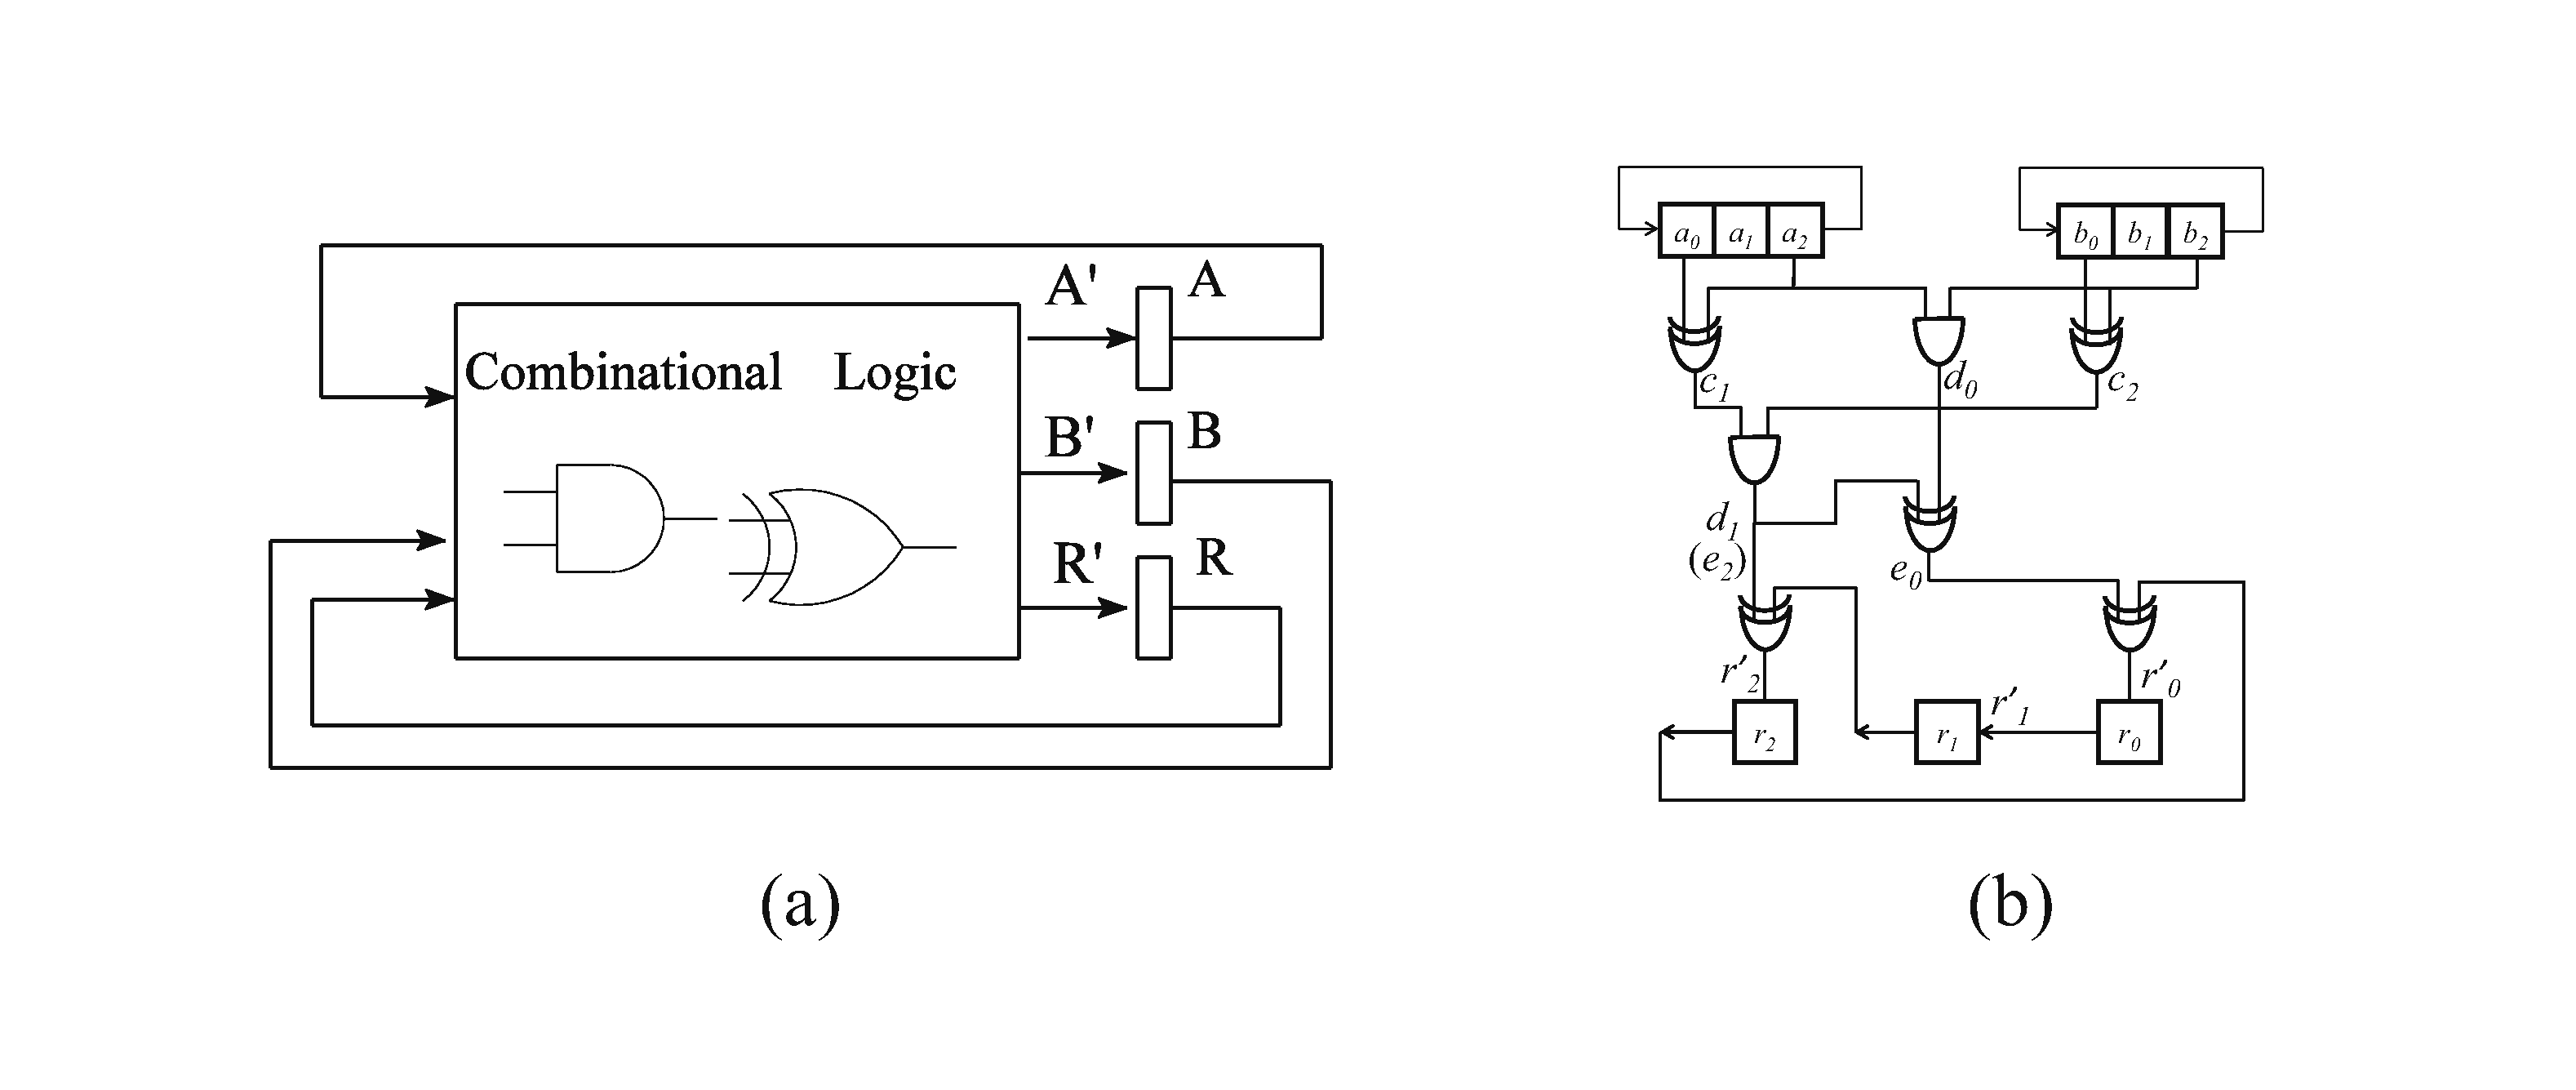
\includegraphics[width=5.5in]{./new_multi.eps}
% \vspace{-0.2in}
\caption{A 3-bit RH-SMPO and its Moore FSM model}
%\end{minipage}
\label{fig:RHmulti}}
\end{figure}
\end{frame}
%%%%%%%%%%%%%%%%%%%%%%%%%%%%%%%%%%%%%%%%%%%%%%%%%%%%%%%%%%%
\begin{frame}{\large{Our approach vs Conventional approach}}
\vspace{-0.1in}
\begin{figure}[H]
\centering{
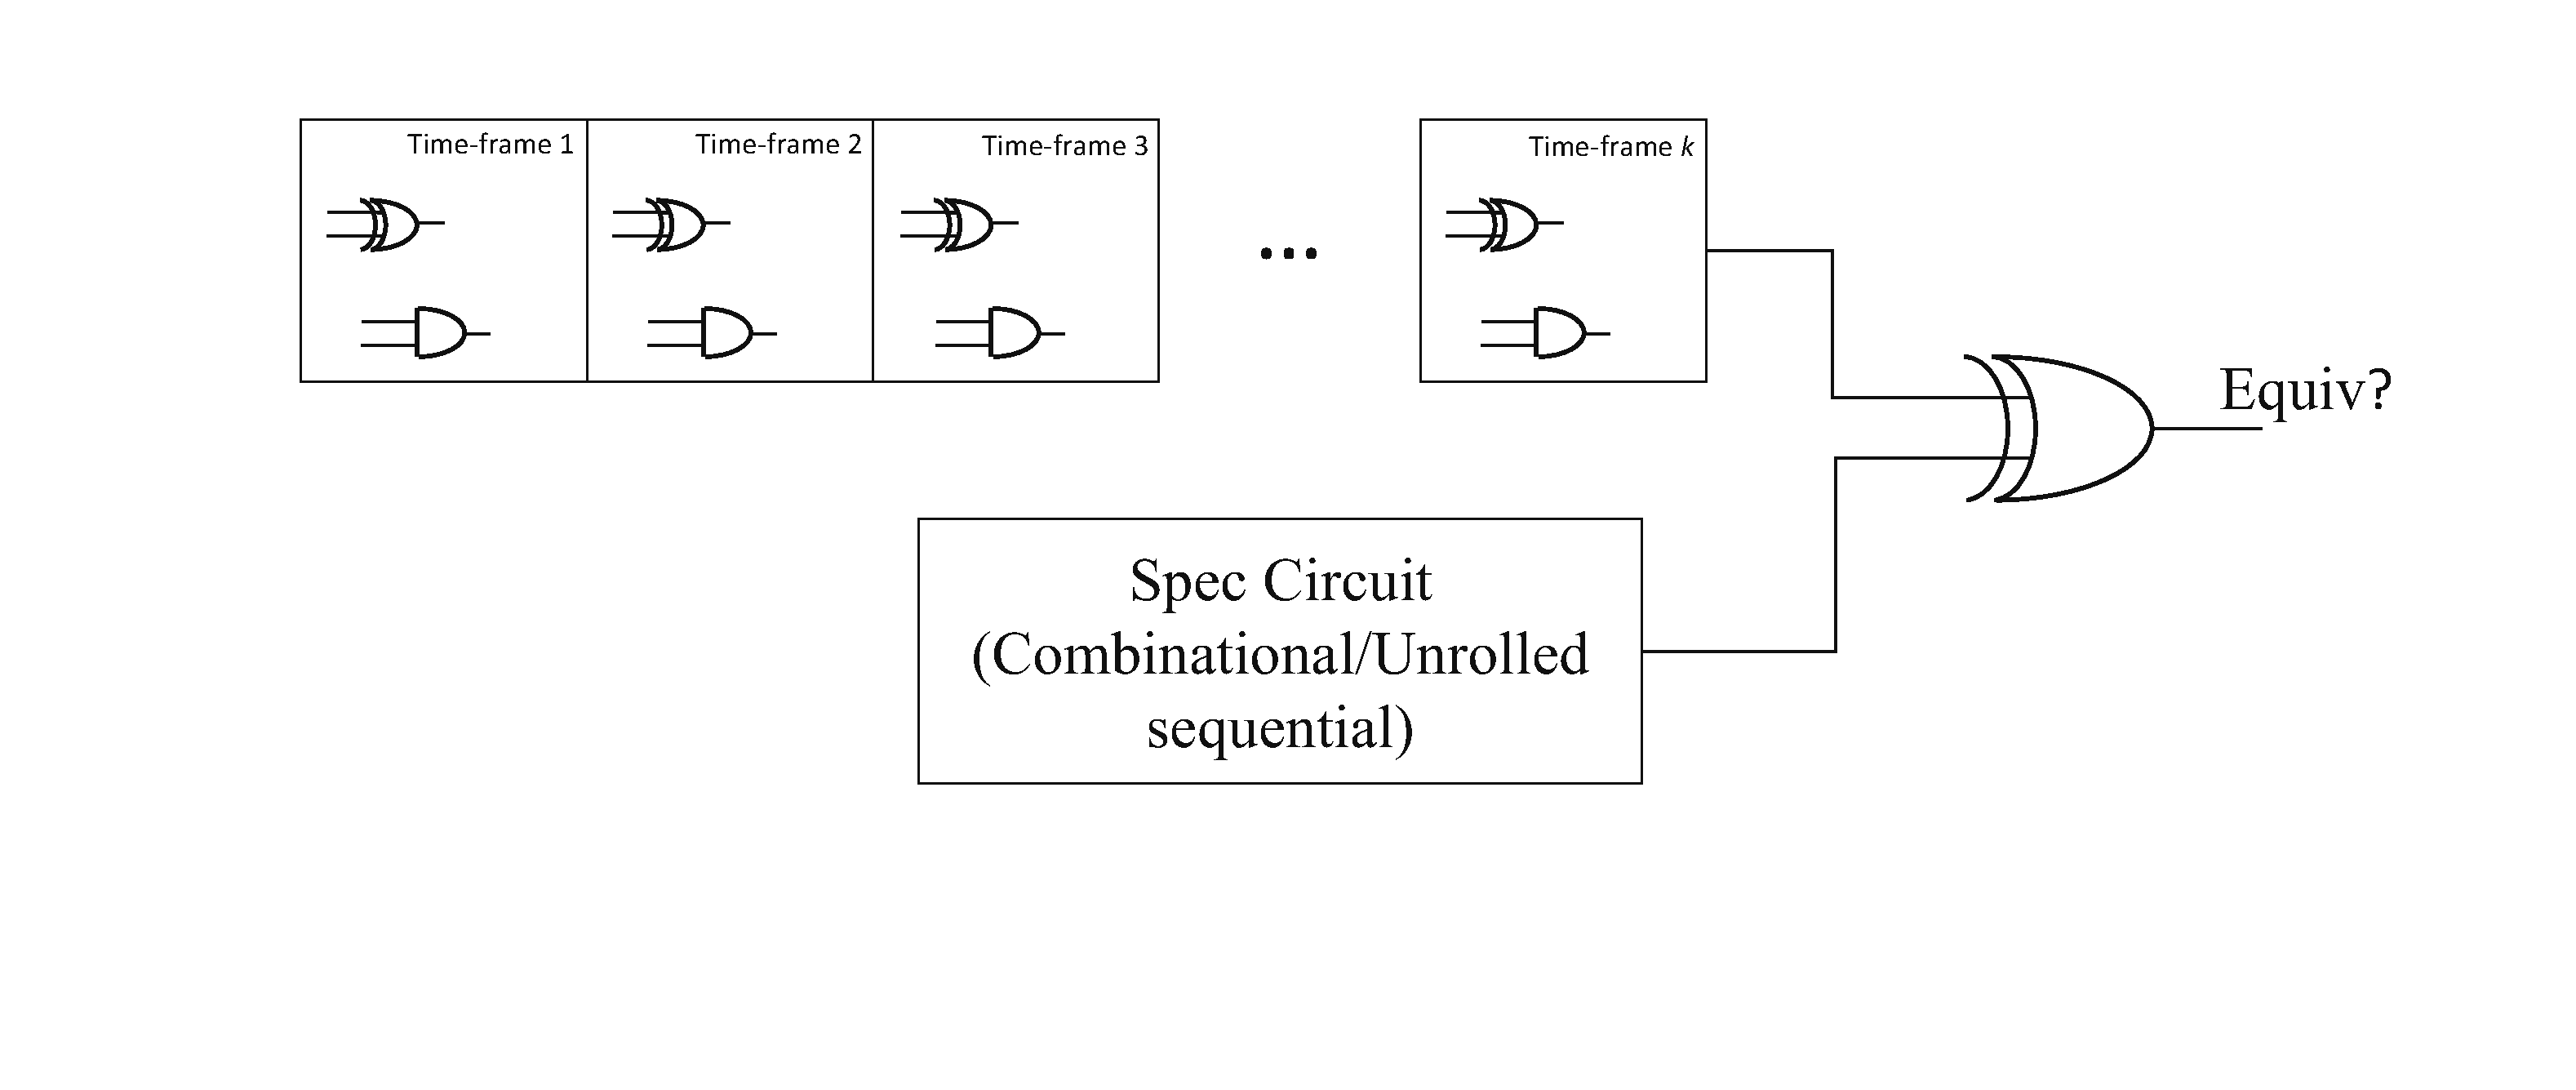
\includegraphics[width=4.5in]{./convention.eps}
}
\end{figure}
\vspace{-0.4in}
\bi
\item Conventional: explicitly unroll $k$ time-frames
	\bi
	\item Bit-blasting!
	\ei
\item New: \alert{Implicitly} unroll
	\bi
	\item Keep only $k$ polynomials ($R = \F(A,B)$) when unrolling
	\item $R_1 = \F(A_{init},B_{init}),~R_2 = \F(A_{1},B_{1}) = \F^2(A_{init},B_{init}),~ 
	\cdots, ~ R_k = \F^k(A_{init},B_{init}) = A_{init}\cdot B_{init}$
	\ei
\ei
\end{frame}
%%%%%%%%%%%%%%%%%%%%%%%%%%%%%%%%%%%%%%%%%%%%%%%%%%%%%%%%%
\begin{frame}{\large{Experiment results}}
\begin{table}[htb]
\centering
\caption{\small Run-time (seconds) for verification of bug-free and
  buggy RH-SMPO using our approach} 
\label{tbl:exp1}  
\begin{tabular}{|c||c|c|c|c|c|c|} 
\hline
Operand size $k$ & 33 & 51 & 65 & 81 & 89 & 99\\
\hline
\#variables & 4785 & 11424 & 18265 & 28512 & 34354 & 42372\\
\hline
\#polynomials & 3630 & 8721 & 13910 & 21789 & 26255 & 32373\\
\hline
\#terms & 13629 & 32793 & 52845 & 82539 & 99591 & 122958\\
\hline
\hline
Runtime(bug-free) & 112.6 & 1129 & 5243 & 20724 & 36096 & 67021\\
\hline
Runtime(buggy) & 112.7 & 1129 & 5256 & 20684 & 36120 & 66929\\
\hline
\end{tabular}
\end{table}
* \textit{Results from X. Sun, et al. ``Formal Verification of Sequential Galois Field Arithmetic 
Circuits using Algebraic Geometry", to be presented in Grenoble, DATE'15}
\end{frame}
%%%%%%%%%%%%%%%%%%%%%%%%%%%%%%%%%%%%%%%%%%%%%%%%%%%%%%%%%
\begin{frame}{\large{What I have done for this experiment}}
\bi
\item Sequential arithmetic circuits over normal basis
\item Standard basis $\rightleftharpoons$ normal basis
\item Optimal normal basis
\item Design circuit(multiplier) over optimal normal basis
\item Verify the function of the circuit
\ei
\hyperlink{pptnodetail}{\beamergotobutton{No more details!}}
\end{frame}
%%%%%%%%%%%%%%%%%%%%%%%%%%%%%%%%%%%%%%%%%%%%%%%%%%%%%%%%%%
\begin{frame}{\large{Normal basis representation}}
\bi
\item Normal basis representation: $A(a_0,\dots,a_{k-1}) = \sum_{i=0}^{k-1}a_{n(i)}\beta^{2^i}$
\item Normal element: $\beta = \alpha^t$
\item Squaring of elements represented in
normal bases can be implemented simply by a cyclic right-shift
operation.
\ei
\begin{Example}
\label{ex:nb_sq}
For $a, b \in \Fkk, (a+b)^2 = a^2 + b^2$. Applying this rule for
element squaring: 
\begin{align}
B = & (b_0\beta + b_1\beta^2 + b_2\beta^4 + \dots + b_{k-1}\beta^{2^{k-1}}) \nonumber\\
B^2 = &b_0^2\beta^2 + b_1^2\beta^4 + b_2^2\beta^8 + \dots + b_{k-1}^2\beta^{2^k} \nonumber\\
= &b_{k-1}\beta + b_0\beta^2 + b_1\beta^4 + \dots + b_{k-2}\beta^{2^{k-1}} \nonumber
\end{align}
as $\beta^{2^k} = \beta$ by applying Fermat's little theorem to $\Fkk$, and $b_i^2 = b_i$. 
\end{Example}
\end{frame}
%%%%%%%%%%%%%%%%%%%%%%%%%%%%%%%%%%%%%%%%%%%%%%%%%%%%%%%%%%%%%%
\begin{frame}{\large{Galois field multiplication with normal basis}}
\bi
\item Let $R =
\sum_{i=0}^{k-1} r_i \beta^{2^{i}}, ~A = \sum_{i=0}^{k-1} a_i
\beta^{2^{i}}, ~B = \sum_{i=0}^{k-1} b_i \beta^{2^{i}}$, then 
\[
R = A\cdot B = (\sum_{i=0}^{k-1} a_i \beta^{2^{i}}) (\sum_{j=0}^{k-1}
b_j \beta^{2^{j}})  =
\sum_{i=0}^{k-1}\sum_{j=0}^{k-1}a_ib_j\beta^{2^i}\beta^{2^j}\nonumber 
\]

\item Expressions $\beta^{2^i}\beta^{2^j}$ are called cross-product
terms. Their normal basis representations are: 
\begin{displaymath}
\beta^{2^i}\beta^{2^j} =
\sum_{n=0}^{k-1}\lambda_{ij}^{(n)}\beta^{2^n}, \ \ \lambda_{ij}^{(n)}
\in \mathbb F_2. 
\end{displaymath}
\ei
\end{frame}
\begin{frame}{\large{Galois field multiplication with normal basis(2)}}
\bi
\item The expression for the
$n^{th}$ digit of product $R = (r_0, \dots, r_n, \dots r_{k-1})$ is:
\[
r_n = \sum_{i=0}^{k-1}\sum_{j=0}^{k-1}\lambda_{ij}^{(n)}a_ib_j = A
\cdot M_n \cdot B^T, ~~0 \leq n \leq k-1
\]
\item $M_n = (\lambda_{ij}^{(n)})$ is a binary $k \times k$ matrix over
$\mathbb F_2$, and it is called the $\lambda$-matrix. 
\item $\lambda$-matrix is \alert{unique} when $k$ and $\beta$ are given!
\ei
\end{frame}

%%%%%%%%%%%%%%%%%%%%%%%%%%%%%%%%%%%%%%%%%%%%%%%%%%%%%%%%%%%
\begin{frame}{\large{Modified algorithm to verify the function of sequential GF multipliers}}
\begin{algorithm}[H] % note [hbt] will fail in beamer
\SetAlgoNoLine
 \KwIn{Circuit polynomial ideal $J$, vanishing ideal $J_0$, initial state ideal $R (=0), \mathcal{G}(A_{init}), \mathcal{H}(B_{init})$} 

  $from_0(R,A,B) = \langle R, \mathcal{G}(A_{init}), \mathcal{H}(B_{init})\rangle$\;
  $i = 0$\;
  \Repeat{$i == k$}
  {
  	$i \gets i + 1$\;
	$G \gets$GB$( \langle J + J_0+ from_{i-1}(R,A,B) \rangle)$ with ATO\;
	$to_i(R',A',B')\gets G\cap \mathbb F_{2^k}[R',A',B',R,A,B]$\;
	$from_i \gets to_i(\{R,A,B\}\setminus \{R',A',B'\})$\;
  }
\Return{$from_k(R_{final})$}
\caption {Abstraction via implicit unrolling for Sequential GF circuit verification}
\end{algorithm}
\end{frame}
%%%%%%%%%%%%%%%%%%%%%%%%%%%%%%%%%%%%%%%%%%%%%%%%%%%%%%%%%%
\begin{frame}{\large{Experiment on 3-bit RH-SMPO}}
\begin{figure}[hbt]
\centering{
%\begin{minipage}{12cm}
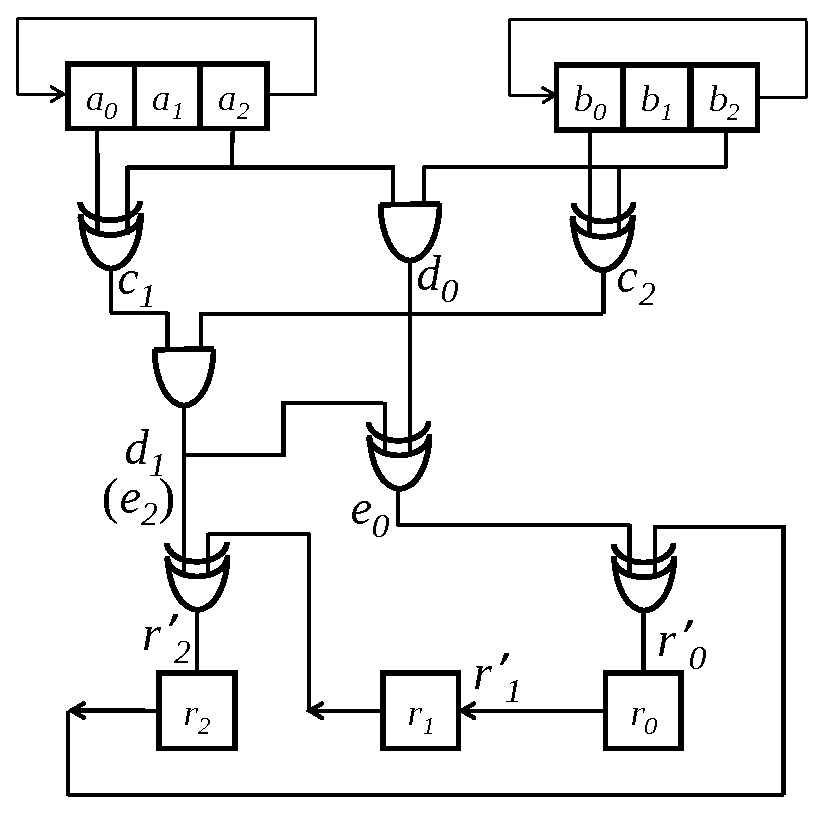
\includegraphics[width=1.5in]{./RH3.eps}
% \vspace{-0.2in}
%\caption{Gate-level circuit of 3-bit RH-SMPO}
%\end{minipage}
\label{fig:RHmulti}}
\end{figure}
\vspace{-0.2in}
\bi
\item The elimination ideal (first iteration):
\begin{align*}
J = &d_0+b_2\cdot a_2,
c_1+a_0+a_2,
c_2+b_0+b_2,
d_1+c_1\cdot c_2,\\
&e_0+d_0+d_1,
e_2+d_1,
r_0'+r_2+e_0,
r_1'+r_0,
r_2'+r_1+e_2,\\
&A+a_0\alpha^3+a_1\alpha^6+a_2\alpha^{12},
B+b_0\alpha^3+b_1\alpha^6+b_2\alpha^{12},\\
&R+r_0\alpha^3+r_1\alpha^6+r_2\alpha^{12},
R'+r_0'\alpha^3+r_1'\alpha^6+r_2'\alpha^{12};
\end{align*}
\ei
\end{frame}
%%%%%%%%%%%%%%%%%%%%%%%%%%%%%%%%%%%%%%%%%%%%%%%%%%%%%%%%%%%
\begin{frame}{\large{Experiment on 3-bit RH-SMPO(2)}}
\bi
\item ``$J_0$" is the ideal of vanishing polynomials in all bit-level
variables (e.g. $a_0^2-a_0$) and word-level variables (e.g. $A^8-A$).
\item $from_0 = \{R, A_{init}+a_0\alpha^3+a_1\alpha^6+a_2\alpha^{12},
B_{init}+b_0\alpha^3+b_1\alpha^6+b_2\alpha^{12}\}$
\item $to_1 : 
R'+(\alpha^2) A_{init}^4 B_{init}^4+(\alpha^2+\alpha) A_{init}^4 B_{init}^2+(\alpha^2+\alpha) A_{init}^4 B_{init}+(\alpha^2+\alpha) A_{init}^2 B_{init}^4+(\alpha^2+\alpha+1) A_{init}^2 B_{init}^2+(\alpha^2) A_{init}^2 B_{init}+(\alpha^2+\alpha) A_{init} B_{init}^4+(\alpha^2) A_{init} B_{init}^2
$
\item $from_1 = \{
R'+(\alpha^2) A_{init}^4 B_{init}^4+(\alpha^2+\alpha) A_{init}^4 B_{init}^2+(\alpha^2+\alpha) A_{init}^4 B_{init}+(\alpha^2+\alpha) A_{init}^2 B_{init}^4+(\alpha^2+\alpha+1) A_{init}^2 B_{init}^2+(\alpha^2) A_{init}^2 B_{init}+(\alpha^2+\alpha) A_{init} B_{init}^4+(\alpha^2) A_{init} B_{init}^2
, A_{init}+a_2\alpha^3+a_0\alpha^6+a_1\alpha^{12},
B_{init}+b_2\alpha^3+b_0\alpha^6+b_1\alpha^{12}\}$
\item $\cdots$
\item After 3 iterations: $to_3 = \{ \alert{R'+A_{init}B_{init},}
~A_{init}+a_0'\alpha^3+a_1'\alpha^6+a_2'\alpha^{12},
~B_{init}+b_0'\alpha^3+b_1'\alpha^6+b_2'\alpha^{12}\}$
\ei
\end{frame}
%%%%%%%%%%%%%%%%%%%%%%%%%%%%%%%%%%%%%%%%%%%%%%%%%%%%%%%%%%%
%%%%%%%%%%%%%%%%%%%%%%%%%%%%%%%%%%%%%%%%%%%%%%%%%%
\begin{frame}{\large{Outline}}
\bi
\item Introduction
\item Sequential circuit verification requires reachability analysis
\item From bit-level to word-level
\item One step back: Sequential arithmetic circuit verification
\item \alert{New inspiration: UNSAT core extraction using algebraic geometry}
\item The plan
\ei
\end{frame}
%%%%%%%%%%%%%%%%%%%%%%%%%%%%%%%%%%%%%%%%%%%%%%%%%%%


\begin{frame}{\large{An example of abstraction refinement algorithm}}
\begin{algorithm}[H]
\SetAlgoNoLine
	\KwIn{$M$ is the original machine, $p$ is the property to check, $k$ is the number of steps in $k$-BMC}
  $k = $ InitValue\;
  \eIf{$k$-BMC$(M,p,k)$ is \textbf{SAT}}
  {
	\Return{``Found error trace"}
  }
  {
	Extract UNSAT proof $\mathcal P$ of $k$-BMC\;
	$M' = $ \textit{ABSTRACT}$(M,\mathcal P)$\;
  }
  \eIf{MODEL-CHECK$(M',p)$ returns \textbf{PASS}}
  {
	\Return{``Passing property"}
  }
  {
	Increase bound $k$\;
	goto Line 2\;
  }
\caption{$k$-BMC with Abstraction Refinement (L. Zhang Thesis)}
\end{algorithm}
\end{frame}
%%%%%%%%%%%%%%%%%%%%%%%%%%%%%%%%%%%%%%%%%%%%%%%%%%%%%%%%%%%
\begin{frame}{\large{An example of abstraction refinement algorithm(2)}}
\bi
\item $k$-BMC: unroll the machine for $k$ times, represent reachable states with CNF formula to check property $p$
$$I(s_0)\land \bigwedge_{i=0}^{k-1}T(s_i,s_{i+1}) \land \neg p$$
\item UNSAT core: a subset of clauses that is still UNSAT
\item State variables not in UNSAT core: no matter what their values are, $p$ will NOT be violated
\item In abstracted model, ignore these ``irrelevant" variables
\ei
\end{frame}
%%%%%%%%%%%%%%%%%%%%%%%%%%%%%%%%%%%%%%%%%%%%%%%%%%%%%%%%%%%
\begin{frame}{\large{An example of abstraction refinement algorithm(3)}}
\begin{figure}[hbt]
\centering{
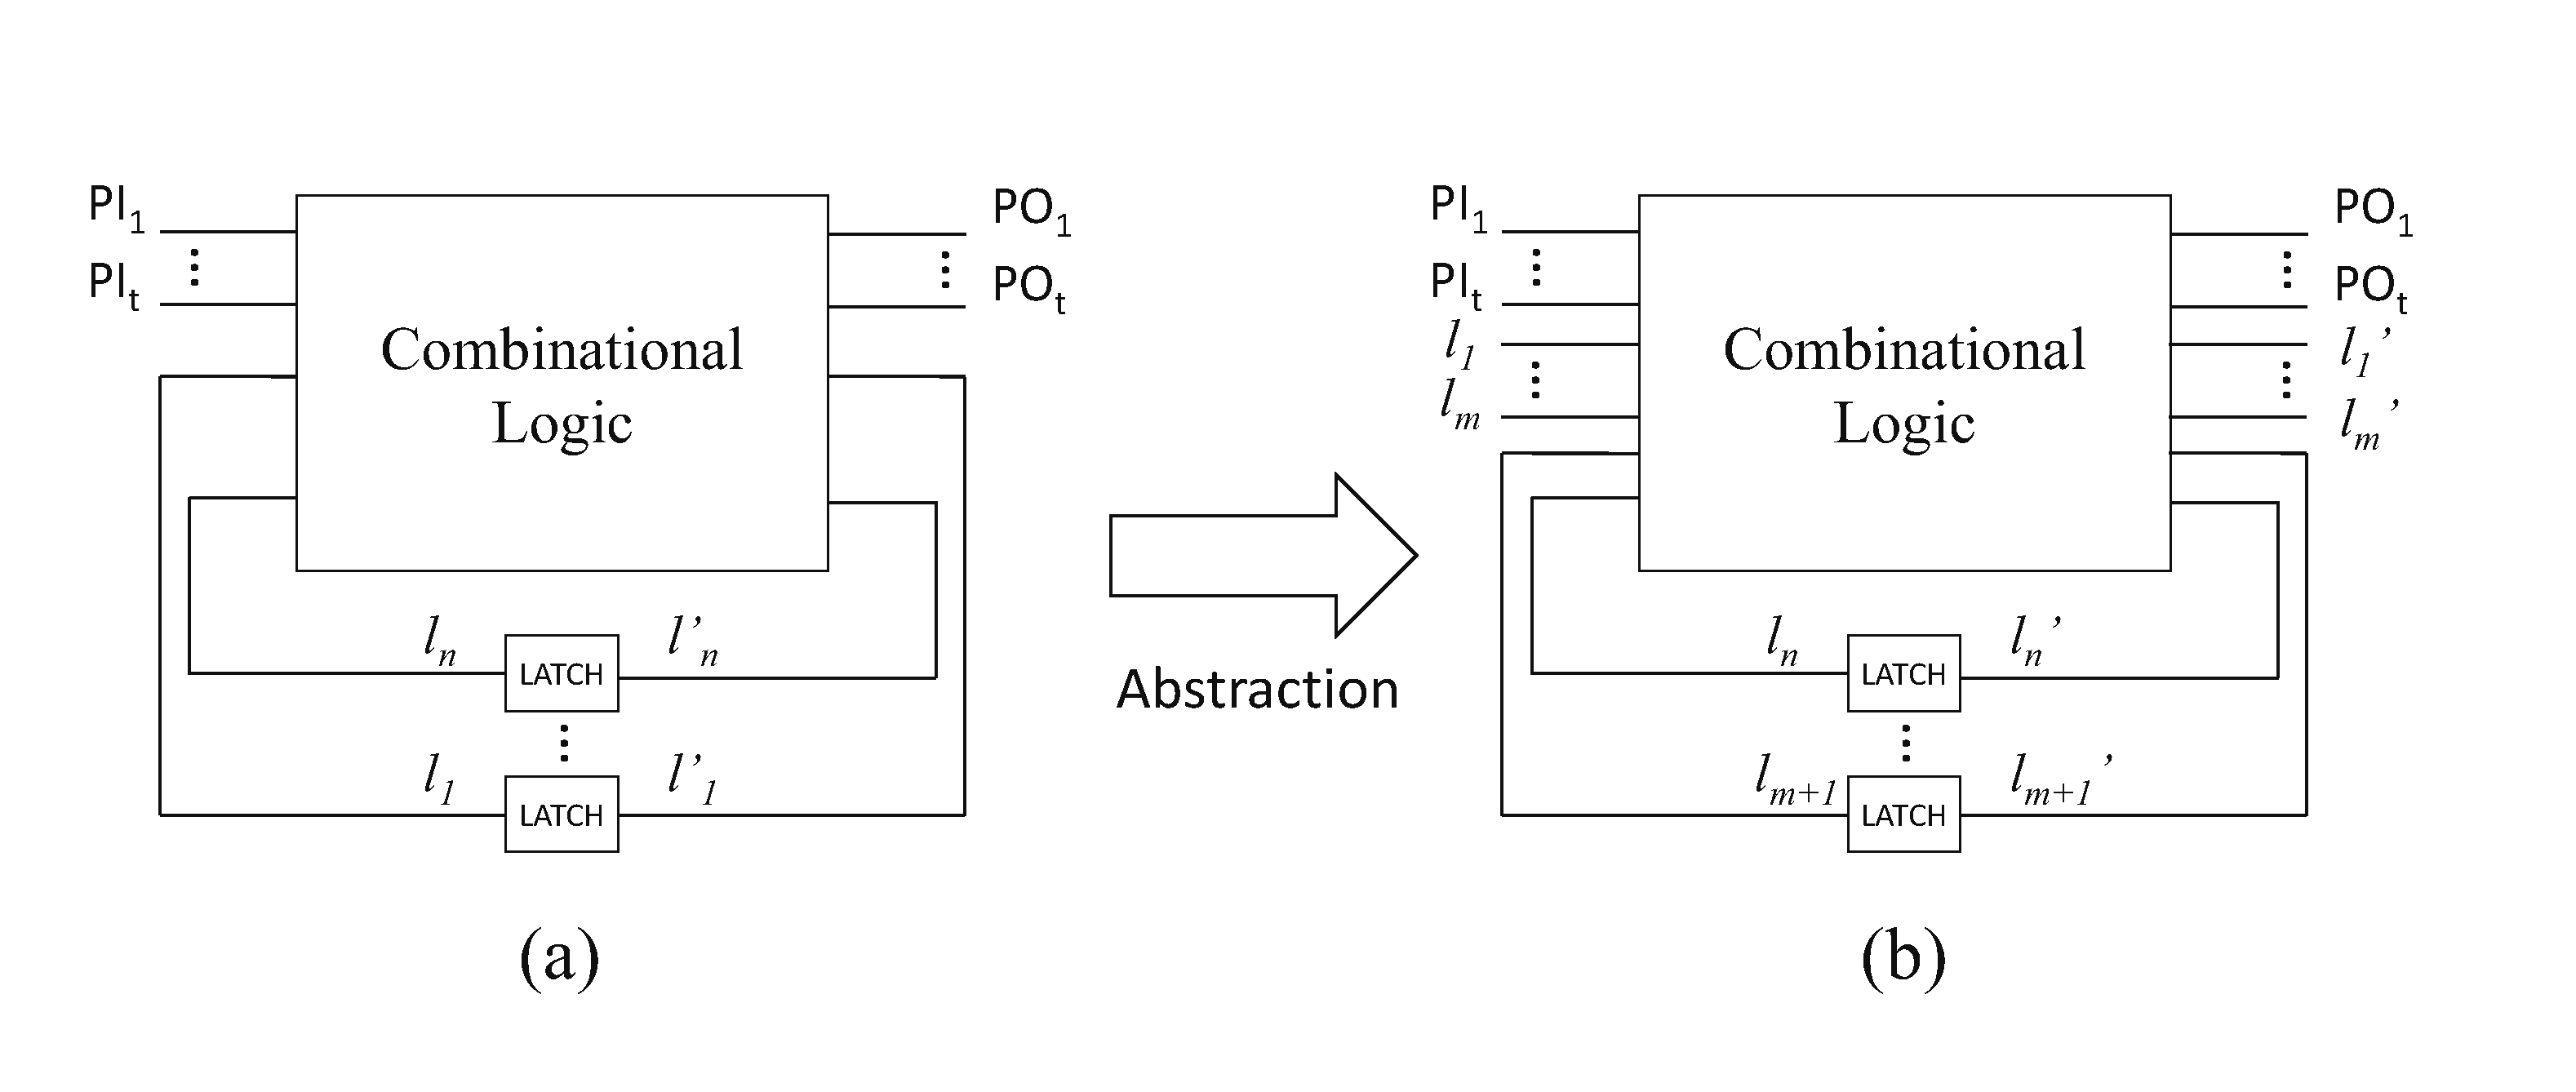
\includegraphics[width=4.5in]{./refine.eps}
\caption{Abstraction by reducing latches}
\label{fig:refine}}
\end{figure}
\bi
\item Remove ``irrelevant" latches, reduce state space
\item Provide an over-approximation
\item This algorithm requires \alert{UNSAT core extraction}
\ei
\end{frame}
%%%%%%%%%%%%%%%%%%%%%%%%%%%%%%%%%%%%%%%%%%%%%%%%%%%%%%%%%%%
\begin{frame}{\large{Buchberger's Algorithm Computes a Gr\"obner Basis}}
\vspace{-0.3in}
%{\small
%\begin{algorithm}
%\caption {Buchberger's Algorithm}
{\bf Buchberger's Algorithm}\\
%\label{alg:gb}
%\begin{algorithmic}
% \REQUIRE : $F = \{f_1, \dots, f_s\}$
 INPUT : $F = \{f_1, \dots, f_s\}$\\
% \ENSURE : $G = \{g_1,\dots ,g_t\}$\\ %, a Gr\"{o}bner basis \\
 OUTPUT : $G = \{g_1,\dots ,g_t\}$\\ %, a Gr\"{o}bner basis \\
  $G:= F$; \\
  REPEAT\\
  \hspace{0.1in} $G' := G$\\
  \hspace{0.1in} For each pair $\{f, g\}, f \neq g$ in $G'$ DO\\
\hspace{0.2in}  $S(f, g) \stackrel{G'}{\textstyle\longrightarrow}_+
r$ \\
\hspace{0.2in}  IF $r \neq 0$ THEN $G:= G \cup \{r\}$ \\
%\hspace{0.2in}  $G(x):=G(x) / x$
UNTIL $G = G'$
%\end{algorithmic}
%\end{algorithm}
\bi
\item S-poly: $S(f,g)=\frac{L}{lt(f)}\cdot f - \frac{L}{lt(g)}\cdot g$\par
$L = \text{LCM}(lm(f), lm(g))$, ~~$lm(f)$: leading monomial of $f$
\item Multivariate division: $f\stackrel{g}{\textstyle\longrightarrow}r:~lm(g)|lm(f)\to r = f-\frac{lt(f)}{lt(g)}g$
\ei
%}

\end{frame}
%%%%%%%%%%%%%%%%%%%%%%%%%%%%%%%%%%%%%%%%%%%%%%%%%%%%%%%%%%%
\begin{frame}{\large{Observation when executing Buchberger's algorithm}}
\bi
\item Translate CNF clauses to polynomials in $\mathbb F_2$
\ei
\begin{columns}[onlytextwidth]
\begin{column}{0.3\textwidth}
\begin{align*}
&c_1: \bar{a}\lor\bar{b}\\
&c_2: a\lor\bar{b}\\
&c_3: \bar{a}\lor b\\
&c_4: a\lor b\\
&c_5: x\lor y\\
&c_6: y\lor z\\
&c_7: b\lor \neg y\\
&c_8: a\lor x\lor \neg z
\end{align*}
\end{column}
\begin{column}{0.3\textwidth}

$$\implies$$
\end{column}
\begin{column}{0.4\textwidth}
\begin{align*}
&f_1:ab\\
&f_2:ab+a\\
&f_3:ab+b\\
&f_4:ab+a+b+1\\
&f_5:xy+y+x+1\\
&f_6:yz+y+z+1\\
&f_7:by+y\\
&f_8:axz+az+xz+z
\end{align*}
\end{column}
\end{columns}
\end{frame}
%%%%%%%%%%%%%%%%%%%%%%%%%%%%%%%%%%%%%%%%%%%%%%%%%%%%%%%%%%%
\begin{frame}{\large{Observation when executing Buchberger's algorithm(2)}}
\bi
\item Compute a GB using Buchberger's algorithm
\item Term ordering: $a>b>x>y>z$
\item
\begin{enumerate}
\item Compute $Spoly(f_1,f_2)\xrightarrow{F}_{+} r_1 = a$
\item Update $F=F\cup r_1$
\item Compute $Spoly(f_1,f_3)\xrightarrow{F}_{+} r_2=b$
\item Update $F=F\cup r_2$
\item Use a directed acyclic graph (DAG) to represent the process to get $r_1,r_2$
\item Compute $Spoly(f_1,f_4) = s_3= a+b+1$, $a+b+1$ can be reduced 
$r_1$ , the intermediate remainder $r_3 = b+1$. Then divided by $r_2$, and the remainder is ``1", 
\alert{terminate the Buchberger's algorithm}
\item Draw a DAG depicting the process through which we obtain remainder ``1". 
From leaf ``1" we backtrace the graph to roots $f_1,f_2,f_3,f_4$. 
\end{enumerate}
\ei
\end{frame}
%%%%%%%%%%%%%%%%%%%%%%%%%%%%%%%%%%%%%%%%%%%%%%%%%%%%%%%%%%%
\begin{frame}{\large{Observation when executing Buchberger's algorithm(3)}}
\begin{figure}[H]
\centering{
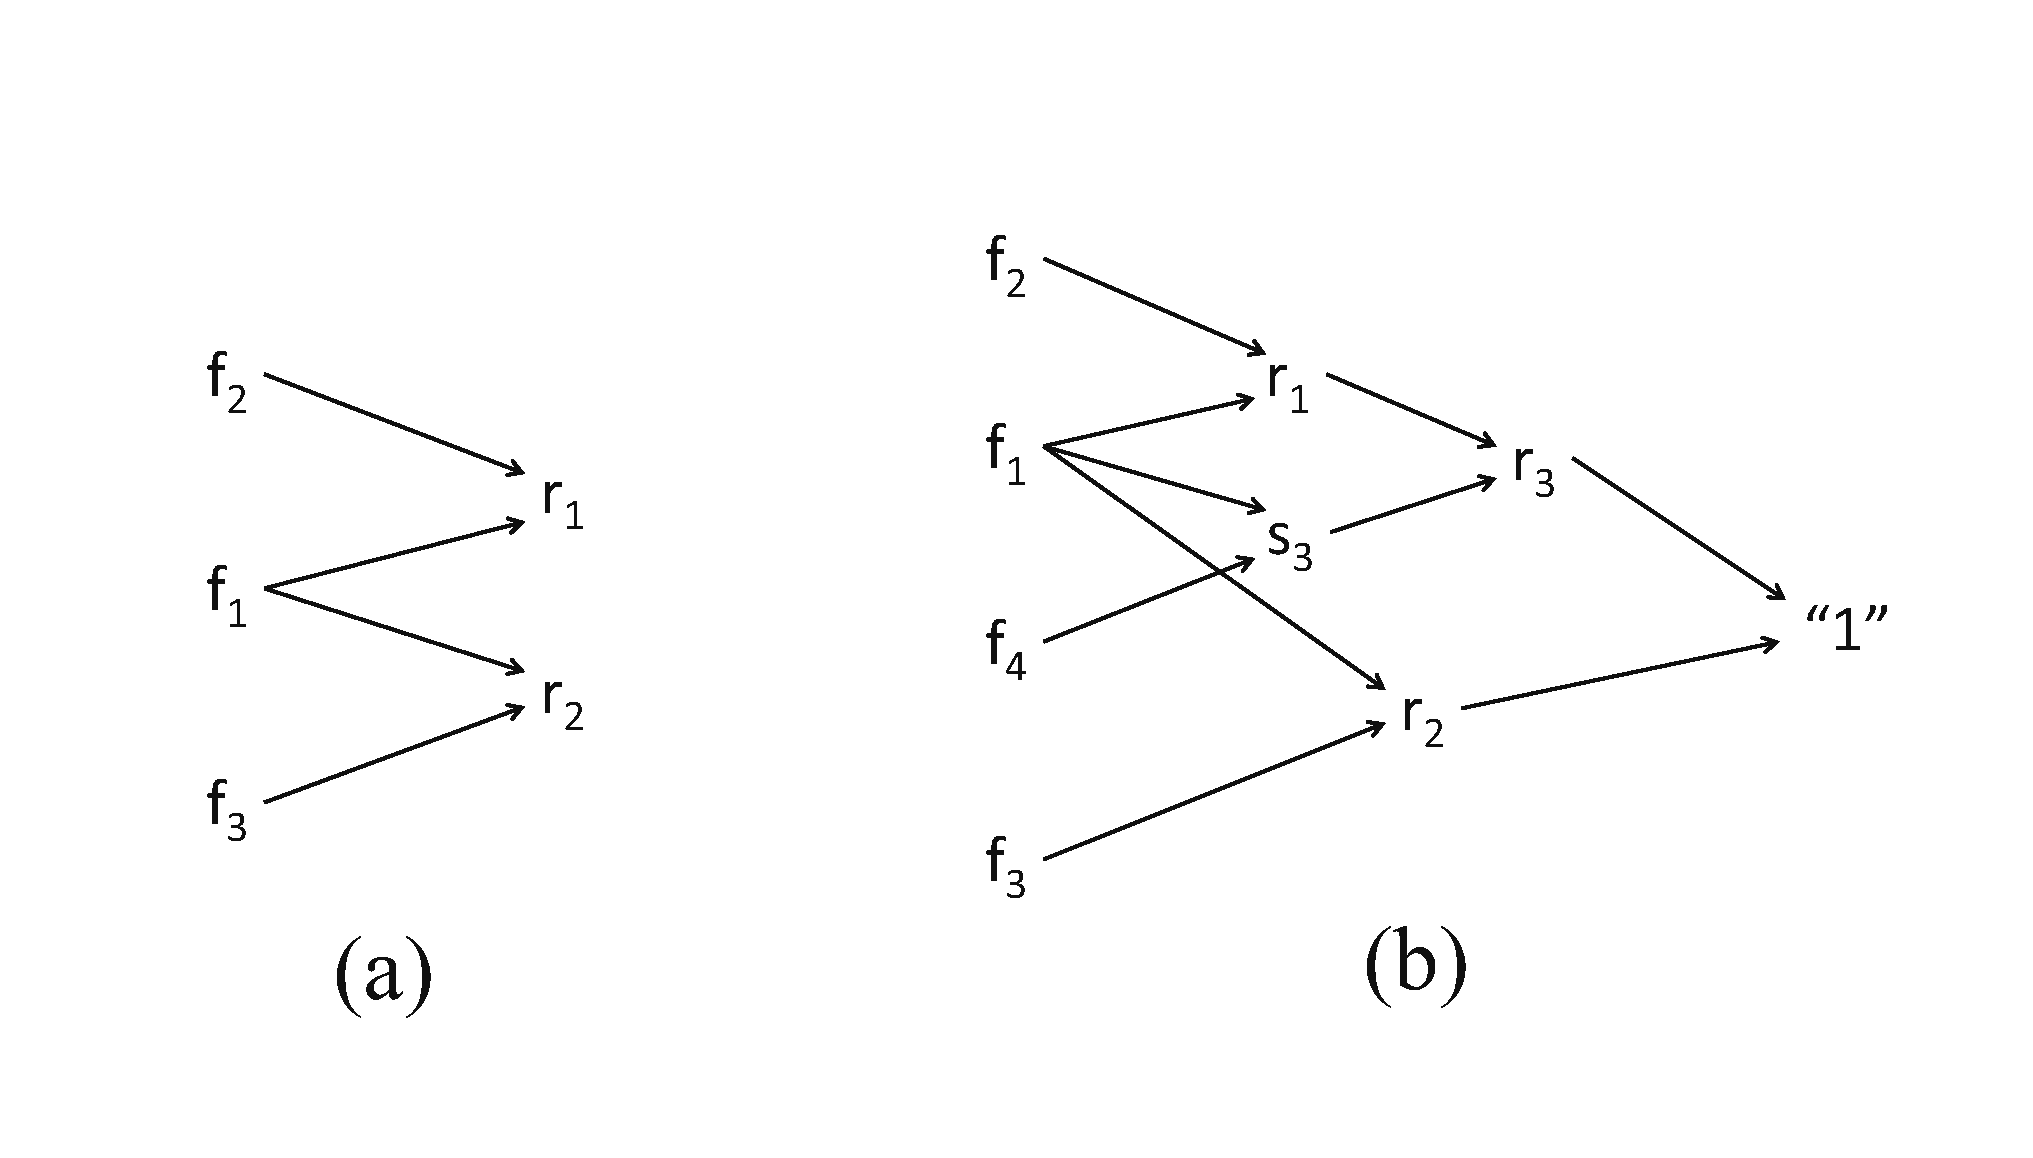
\includegraphics[width=4.5in]{./UNSAT.eps}
\caption{DAG representing Spoly computations and multivariate divisions}
\label{fig:UNSAT}}
\end{figure}
\end{frame}
%%%%%%%%%%%%%%%%%%%%%%%%%%%%%%%%%%%%%%%%%%%%%%%%%%%%%%%%%%%
\begin{frame}{\large{Observation when executing Buchberger's algorithm(3)}}
\begin{figure}[H]
\centering{
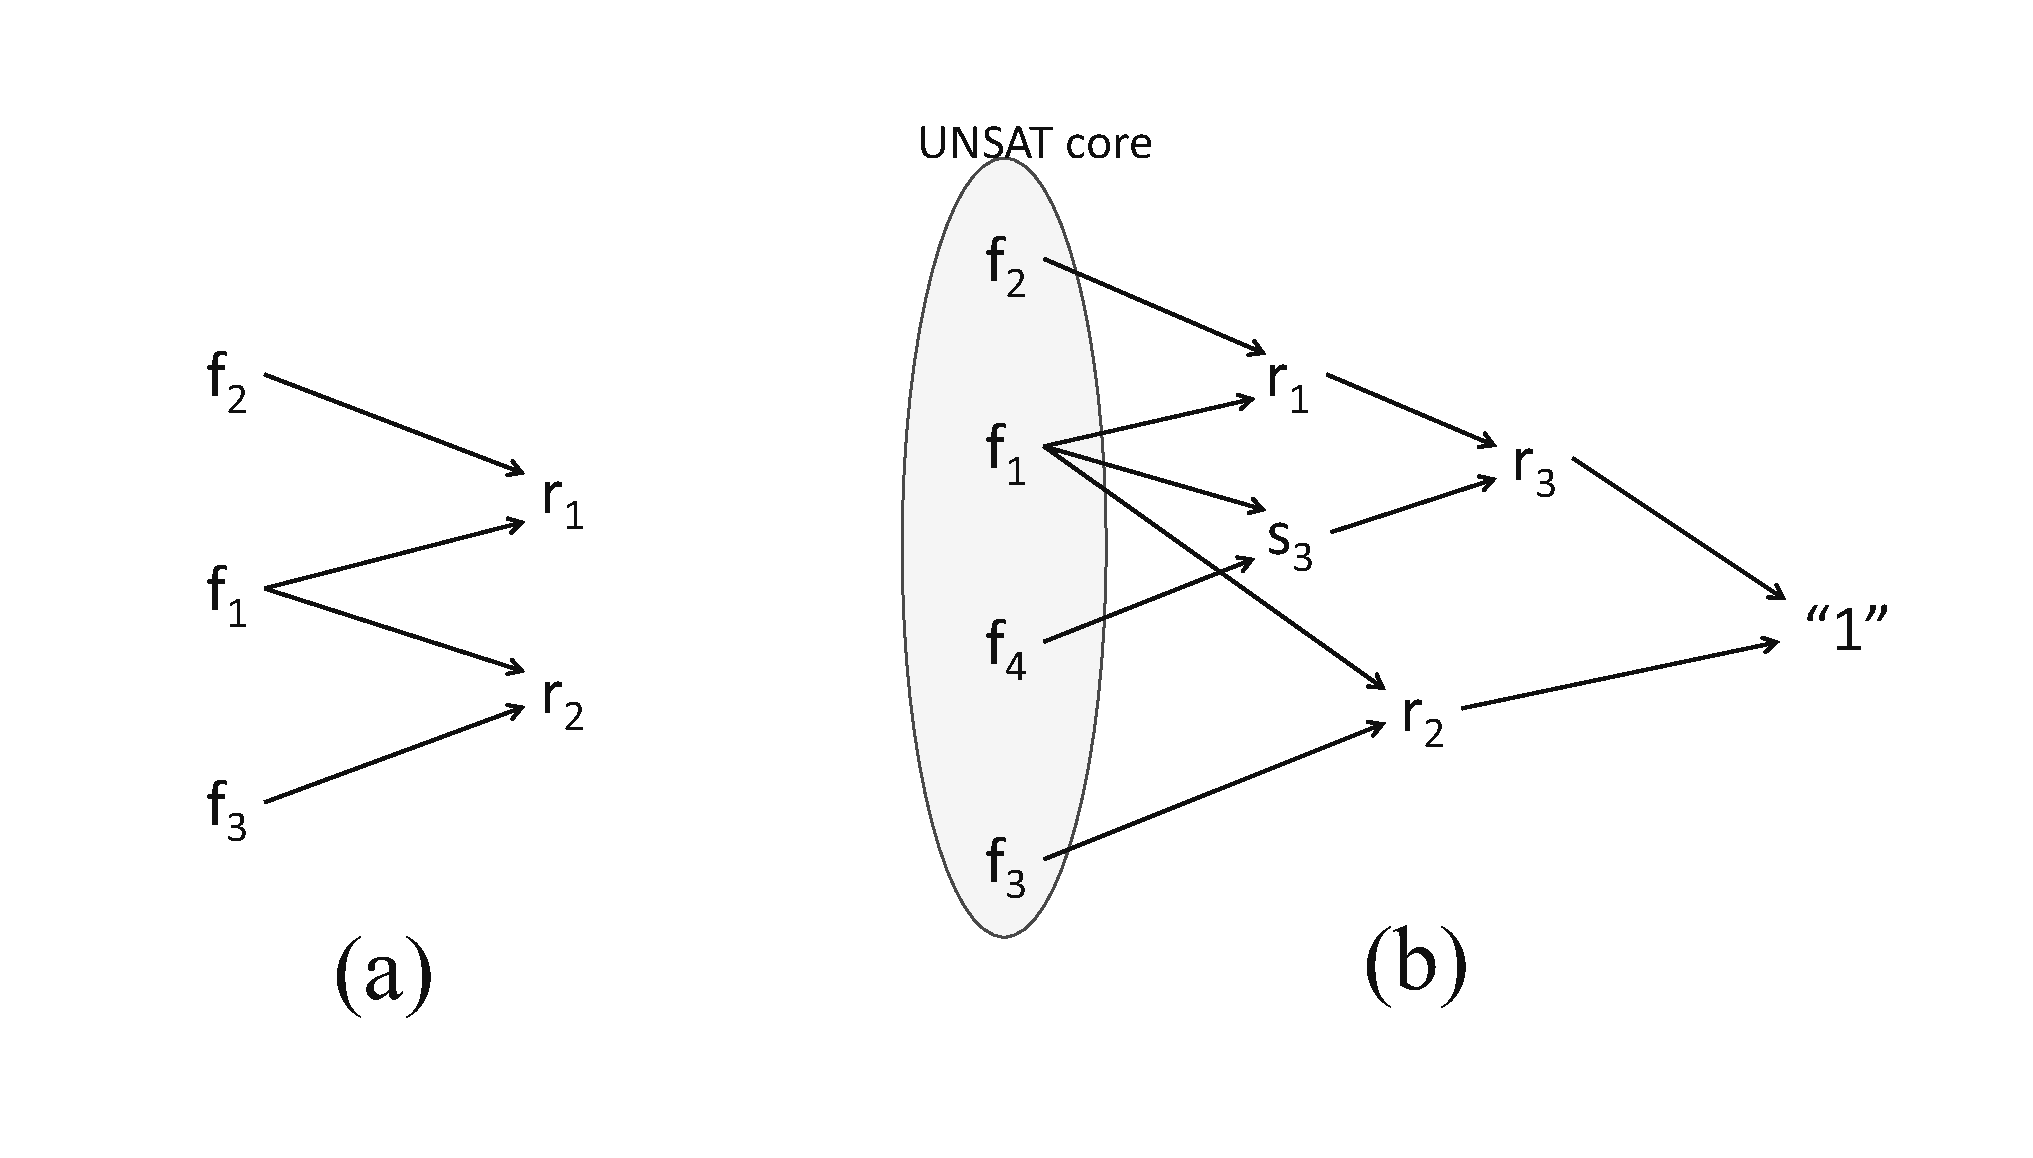
\includegraphics[width=4.5in]{./UNSAT2.eps}
\caption{DAG representing Spoly computations and multivariate divisions}
}
\end{figure}
\end{frame}
%%%%%%%%%%%%%%%%%%%%%%%%%%%%%%%%%%%%%%%%%%%%%%%%%%%%%%%%%%%
\begin{frame}{\large{Proposed algorithm to extract UNSAT core}}
\begin{algorithm}[H]
\SetAlgoNoLine
	\KwIn{A set of polynomials $F = \{f_1,f_2,\dots,f_s\}$}
	\KwOut{An UNSAT core $\{f_{m_1},f_{m_2},\dots,f_{m_t}\}$}
\Repeat{$r_l == 1$}
{
	Pick a pair $f_i,f_j\in F$ that has never been computed S-poly\;
	\If{$Spoly(f_i,f_j)\xrightarrow{F}_+ r_l \neq 0$}
	{
		$F = F\cup r_l$\;
		Create a DAG $G_l$ with $f_i,f_j$ as roots, $r_l$ as leaf, recording the S-poly, all intermediate remainders and $f_k\in F$ that cancel monomial terms in the S-poly\;
	}
}
Backward traverse the DAG for remainder ``1", replace $r_l$ with corresponding DAG $G_l$\;
\Return{All roots}
\caption {Extract UNSAT core using a variation of Buchberger's algorithm}
\end{algorithm}
\end{frame}

%%%%%%%%%%%%%%%%%%%%%%%%%%%%%%%%%%%%%%%%%%%%%%%%%%
\begin{frame}{\large{Outline}}
\bi
\item Introduction
\item Sequential circuit verification requires reachability analysis
\item From bit-level to word-level
\item One step back: Sequential arithmetic circuit verification
\item New inspiration: UNSAT core extraction using algebraic geometry
\item \alert{The plan}
\ei
\end{frame}
%%%%%%%%%%%%%%%%%%%%%%%%%%%%%%%%%%%%%%%%%%%%%%%%%%%
%%%%%%%%%%%%%%%%%%%%%%%%%%%%%%%%%%%%%%%%%%%%%%%%%%%%%%%%%%%
\begin{frame}{\large{Objectives}}
\bi
\item Explore an implementation of algebraic geometry based reachability analysis
\item CAD tool design
	\bi
	\item {\sc Singular}'s data structure not optimized $\to$ design a standalone CAD tool implemented in C++
	\item Specifically aims to solve word-level sequential verification problems
	\item Lower complexity: borrow techniques from [T. Pruss, {\it Abstraction}, DAC'14], [J. Lv, {\it Equivalence}, TCAD'13]
		and [C. Eder, {\it F-4 reduction}, ISSAC'11]
	\ei
\item Fine-tune the tool for sequential GF arithmetic circuits verification
\item Explore a new abstraction-refinement paradigm based on information from UNSAT cores
\ei
\end{frame}
%%%%%%%%%%%%%%%%%%%%%%%%%%%%%%%%%%%%%%%%%%%%%%%%%%%%%%%%%%%
\begin{frame}{\large{Time table}}
\begin{itemize}
\item Current status: Experiments have been performed to run implicit state enumeration on sequential circuits benchmarks
such as ISCAS'89 circuits. Current problem is the algorithm spends too much time on multivariate division procedure;
\item Spring 2015: Implement the tool which can efficiently do multivariate division and test the performance of 
our tool based on [Tim, {\it Abstraction}, DAC'14] approach;
\item Summer 2015: Integrate the refined multivariate division routine into our verification tool, test its
performance on circuits with various sizes;
\item Fall 2015: Evaluate data and write the dissertation.
\end{itemize}
\end{frame}
%%%%%%%%%%%%%%%%%%%%%%%%%%%%%%%%%%%%%%%%%%%%%%%%%%%%%%%%%%%
% \begin{frame}{\large{Obviate GB computation}}
% 
% \end{frame}



\end{document}